% This is a modified version of the tufte-latex book example in which the title page and the contents page resemble Tufte's VDQI book, using Kevin Godby's code from this thread at https://groups.google.com/forum/#!topic/tufte-latex/ujdzrktC1BQ.

%% Unfortunately for the contents to contain
%% the "Parts" lines successfully, hyperref
%% needs to be disabled.
\documentclass[nohyper,nobib,a4]{tufte-book}
\usepackage{nameref}
% \hypersetup{colorlinks}% uncomment this line if you prefer colored hyperlinks (e.g., for onscreen viewing)

% \usepackage{hyphenat}
\usepackage{url}
\usepackage[backend=biber, natbib=true, style=numeric]{biblatex}
\addbibresource{../ZoteroLibUpdated/ZoteroLibUpdated.bib}
\usepackage{xargs}

% from me: Remove the visited on https://tex.stackexchange.com/questions/400384/how-to-disable-biblatex-showing-visited-on-on-the-references
\AtEveryBibitem{
    \clearfield{urlyear}
    \clearfield{urlmonth}
}

% from me: short citation in sideline: https://tex.stackexchange.com/questions/414716/options-for-styling-fullcite
\DeclareCiteCommand{\fullcite}
  {\usebibmacro{prenote}}
  {\clearfield{url}%
   \clearfield{pages}%
   \clearfield{pagetotal}%
   \clearfield{edition}%
       \clearfield{labelyear}%
        \clearfield{doi}%
    \clearfield{labelyear}%
       \clearfield{urlyear}
    \clearfield{urlmonth}
      \clearfield{eprinttype}
      \clearfield{eprint}
      \clearfield{issn}
      \clearfield{volume}
      \clearfield{journaltitle}
       \clearfield{number}
       \clearfield{date}
   \usedriver
     {\DeclareNameAlias{sortname}{default}}
     {\thefield{entrytype}}}
     \multicitedelim
  {\usebibmacro{postnote}}
  %disable side bar
%\renewcommandx{\cite}[3][1={0pt},2={}]{\sidenote[][#1]{\fullcite[#2]{#3}}}

%%
% Book metadata
\title{Modelling and control of infectious disease dynamics}
\date{\today}
\author[Joseph Lemaitre]{Joseph \ Lemaitre}
\publisher{Under the supervision of Prof. Andrea Rinaldo and Dr. Damiano Pasetto.}

%\usepackage{microtype}

%%
% Just some sample text
\usepackage{lipsum}

%%
% For nicely typeset tabular material
\usepackage{booktabs}

%%
% For graphics / images
\usepackage{graphicx}
\setkeys{Gin}{width=\linewidth,totalheight=\textheight,keepaspectratio}
\graphicspath{{graphics/}}

% The fancyvrb package lets us customize the formatting of verbatim
% environments.  We use a slightly smaller font.
\usepackage{fancyvrb}
\fvset{fontsize=\normalsize}

%%
% Prints argument within hanging parentheses (i.e., parentheses that take
% up no horizontal space).  Useful in tabular environments.
\newcommand{\hangp}[1]{\makebox[0pt][r]{(}#1\makebox[0pt][l]{)}}

%%
% Prints an asterisk that takes up no horizontal space.
% Useful in tabular environments.
\newcommand{\hangstar}{\makebox[0pt][l]{*}}

%%
% Prints a trailing space in a smart way.
\usepackage{xspace}

%%
% Some shortcuts for Tufte's book titles.  The lowercase commands will
% produce the initials of the book title in italics.  The all-caps commands
% will print out the full title of the book in italics.
\newcommand{\vdqi}{\textit{VDQI}\xspace}
\newcommand{\ei}{\textit{EI}\xspace}
\newcommand{\ve}{\textit{VE}\xspace}
\newcommand{\be}{\textit{BE}\xspace}
\newcommand{\VDQI}{\textit{The Visual Display of Quantitative Information}\xspace}
\newcommand{\EI}{\textit{Envisioning Information}\xspace}
\newcommand{\VE}{\textit{Visual Explanations}\xspace}
\newcommand{\BE}{\textit{Beautiful Evidence}\xspace}

\newcommand{\TL}{Tufte-\LaTeX\xspace}

% Prints the month name (e.g., January) and the year (e.g., 2008)
\newcommand{\monthyear}{%
  \ifcase\month\or January\or February\or March\or April\or May\or June\or
  July\or August\or September\or October\or November\or
  December\fi\space\number\year
}


% Prints an epigraph and speaker in sans serif, all-caps type.
\newcommand{\openepigraph}[2]{%
  %\sffamily\fontsize{14}{16}\selectfont
  \begin{fullwidth}
  \sffamily\large
  \begin{doublespace}
  \noindent\allcaps{#1}\\% epigraph
  \noindent\allcaps{#2}% author
  \end{doublespace}
  \end{fullwidth}
}

% Inserts a blank page
\newcommand{\blankpage}{\newpage\hbox{}\thispagestyle{empty}\newpage}

\usepackage{units}

% Typesets the font size, leading, and measure in the form of 10/12x26 pc.
\newcommand{\measure}[3]{#1/#2$\times$\unit[#3]{pc}}

% Macros for typesetting the documentation
\newcommand{\hlred}[1]{\textcolor{Maroon}{#1}}% prints in red
\newcommand{\hangleft}[1]{\makebox[0pt][r]{#1}}
\newcommand{\hairsp}{\hspace{1pt}}% hair space
\newcommand{\hquad}{\hskip0.5em\relax}% half quad space
\newcommand{\TODO}{\textcolor{red}{\bf TODO!}\xspace}
\newcommand{\ie}{\textit{i.\hairsp{}e.}\xspace}
\newcommand{\eg}{\textit{e.\hairsp{}g.}\xspace}
\newcommand{\na}{\quad--}% used in tables for N/A cells
\providecommand{\XeLaTeX}{X\lower.5ex\hbox{\kern-0.15em\reflectbox{E}}\kern-0.1em\LaTeX}
\newcommand{\tXeLaTeX}{\XeLaTeX\index{XeLaTeX@\protect\XeLaTeX}}
% \index{\texttt{\textbackslash xyz}@\hangleft{\texttt{\textbackslash}}\texttt{xyz}}
\newcommand{\tuftebs}{\symbol{'134}}% a backslash in tt type in OT1/T1
\newcommand{\doccmdnoindex}[2][]{\texttt{\tuftebs#2}}% command name -- adds backslash automatically (and doesn't add cmd to the index)
\newcommand{\doccmddef}[2][]{%
  \hlred{\texttt{\tuftebs#2}}\label{cmd:#2}%
  \ifthenelse{\isempty{#1}}%
    {% add the command to the index
      \index{#2 command@\protect\hangleft{\texttt{\tuftebs}}\texttt{#2}}% command name
    }%
    {% add the command and package to the index
      \index{#2 command@\protect\hangleft{\texttt{\tuftebs}}\texttt{#2} (\texttt{#1} package)}% command name
      \index{#1 package@\texttt{#1} package}\index{packages!#1@\texttt{#1}}% package name
    }%
}% command name -- adds backslash automatically
\newcommand{\doccmd}[2][]{%
  \texttt{\tuftebs#2}%
  \ifthenelse{\isempty{#1}}%
    {% add the command to the index
      \index{#2 command@\protect\hangleft{\texttt{\tuftebs}}\texttt{#2}}% command name
    }%
    {% add the command and package to the index
      \index{#2 command@\protect\hangleft{\texttt{\tuftebs}}\texttt{#2} (\texttt{#1} package)}% command name
      \index{#1 package@\texttt{#1} package}\index{packages!#1@\texttt{#1}}% package name
    }%
}% command name -- adds backslash automatically
\newcommand{\docopt}[1]{\ensuremath{\langle}\textrm{\textit{#1}}\ensuremath{\rangle}}% optional command argument
\newcommand{\docarg}[1]{\textrm{\textit{#1}}}% (required) command argument
\newenvironment{docspec}{\begin{quotation}\ttfamily\parskip0pt\parindent0pt\ignorespaces}{\end{quotation}}% command specification environment
\newcommand{\docenv}[1]{\texttt{#1}\index{#1 environment@\texttt{#1} environment}\index{environments!#1@\texttt{#1}}}% environment name
\newcommand{\docenvdef}[1]{\hlred{\texttt{#1}}\label{env:#1}\index{#1 environment@\texttt{#1} environment}\index{environments!#1@\texttt{#1}}}% environment name
\newcommand{\docpkg}[1]{\texttt{#1}\index{#1 package@\texttt{#1} package}\index{packages!#1@\texttt{#1}}}% package name
\newcommand{\doccls}[1]{\texttt{#1}}% document class name
\newcommand{\docclsopt}[1]{\texttt{#1}\index{#1 class option@\texttt{#1} class option}\index{class options!#1@\texttt{#1}}}% document class option name
\newcommand{\docclsoptdef}[1]{\hlred{\texttt{#1}}\label{clsopt:#1}\index{#1 class option@\texttt{#1} class option}\index{class options!#1@\texttt{#1}}}% document class option name defined
\newcommand{\docmsg}[2]{\bigskip\begin{fullwidth}\noindent\ttfamily#1\end{fullwidth}\medskip\par\noindent#2}
\newcommand{\docfilehook}[2]{\texttt{#1}\index{file hooks!#2}\index{#1@\texttt{#1}}}
\newcommand{\doccounter}[1]{\texttt{#1}\index{#1 counter@\texttt{#1} counter}}

% Generates the index
\usepackage{makeidx}
\makeindex

%%%% Kevin Godny's code for title page and contents from https://groups.google.com/forum/#!topic/tufte-latex/ujdzrktC1BQ
\makeatletter
\renewcommand{\maketitlepage}{%
\begingroup%
\setlength{\parindent}{0pt}

{\fontsize{24}{24}\selectfont\textit{\@author}\par}

\vspace{1.75in}{\fontsize{36}{54}\selectfont\@title\par}

\vspace{0.5in}{\fontsize{14}{14}\selectfont\textsf{\smallcaps{\@date}}\par}

\vfill{\fontsize{14}{14}\selectfont\textit{\@publisher}\par}

\thispagestyle{empty}
\endgroup
}
\makeatother

\titlecontents{part}%
    [0pt]% distance from left margin
    {\addvspace{0.25\baselineskip}}% above (global formatting of entry)
    {\allcaps{Part~\thecontentslabel}\allcaps}% before w/ label (label = ``Part I'')
    {\allcaps{Part~\thecontentslabel}\allcaps}% before w/o label
    {}% filler and page (leaders and page num)
    [\vspace*{0.5\baselineskip}]% after

\titlecontents{chapter}%
    [4em]% distance from left margin
    {}% above (global formatting of entry)
    {\contentslabel{2em}\textit}% before w/ label (label = ``Chapter 1'')
    {\hspace{0em}\textit}% before w/o label
    {\qquad\thecontentspage}% filler and page (leaders and page num)
    [\vspace*{0.5\baselineskip}]% after
%%%% End additional code by Kevin Godby

%%% Joseph's thesis
% cholera-rainfall
\usepackage{amssymb}
\usepackage{amsbsy}
\usepackage{makecell}

\begin{document}

% Front matter
\frontmatter

% r.1 blank page
% \blankpage

% v.2 epigraphs
% \newpage\thispagestyle{empty}
% \openepigraph{%
% The public is more familiar with bad design than good design.
% It is, in effect, conditioned to prefer bad design, 
% because that is what it lives with. 
% The new becomes threatening, the old reassuring.
% }{Paul Rand%, {\itshape Design, Form, and Chaos}
% }
% \vfill
% \openepigraph{%
% A designer knows that he has achieved perfection 
% not when there is nothing left to add, 
% but when there is nothing left to take away.
% }{Antoine de Saint-Exup\'{e}ry}
% \vfill
% \openepigraph{%
% \ldots the designer of a new system must not only be the implementor and the first 
% large-scale user; the designer should also write the first user manual\ldots 
% If I had not participated fully in all these activities, 
% literally hundreds of improvements would never have been made, 
% because I would never have thought of them or perceived 
% why they were important.
% }{Donald E. Knuth}


% r.3 full title page
%\maketitle

% r.5 contents
%\tableofcontents

%\listoffigures

%\listoftables

% r.7 dedication
%\cleardoublepage
%~\vfill
%\begin{doublespace}
%\noindent\fontsize{18}{22}\selectfont\itshape
%\nohyphenation
%Dedicated to those who appreciate \LaTeX{} 
%and the work of \mbox{Edward R.~Tufte} 
%and \mbox{Donald E.~Knuth}.
%\end{doublespace}
%\vfill
%\vfill


% r.9 introduction
\cleardoublepage
\chapter*{Introduction}


%%
% Start the main matter (normal chapters)
\mainmatter

\part{Modeling of Cholera: rainfall, vaccination}

\chapter{Rainfall as a driver of epidemic cholera: Comparative model assessments of the effect of intra-seasonal precipitation events}
\label{ch:cholera-rainfall}

\begin{fullwidth}
\chapter[Rainfall as a driver of epidemic cholera: Comparative assessments of the effect of intra-seasonal precipitation events]{Rainfall as a driver of epidemic cholera:\\Comparative assessments of the effect of\\intra-seasonal precipitation events}\label{ch:cholera-rainfall}

The correlation between cholera epidemics and climatic drivers, in particular seasonal tropical rainfall, has been studied in a variety of contexts. Several mechanistic models have included rainfall as a driver of cholera transmission by focusing on two possible pathways: either by increasing exposure to contaminated water (\eg due to worsening sanitary conditions during water excess), or by increased water contamination with freshly excreted bacteria (\eg due to washout of open-air defecation sites or overflows). In this chapter, the explanatory power of these different model structures is assessed by formal model comparison using deterministic and stochastic models of the type susceptible-infected-recovered-bacteria (SIRB). The incorporation of rainfall effects is generalized using a nonlinear function that can increase or decrease the relative importance of large precipitation events. The modelling framework is applied on the daily epidemiological data collected during the 2015 cholera outbreak in Juba, South Sudan. This epidemic is characterized by a particular intra-seasonal double peak of incidence in apparent relation with particularly strong rainfall events. Results suggest that rainfall-based models in both their deterministic and stochastic formulations outperform models that do not account for rainfall. In fact, classical SIRB models are not able to reproduce the second peak, suggesting it was rainfall-driven. Moreover stronger support is found for rainfall acting on increased exposure rather than on exacerbated water contamination. Although these results are context-specific, they stress the importance of a systematic and comprehensive appraisal of transmission pathways and their environmental forcings when embarking in the modelling of epidemic cholera.

This section is adapted from:
\longfullcite{Lemaitre:RainfallDriverEpidemic:2019}.%\footnote[][-4\baselineskip]{JL, JP-S and DP developed the numerical tools required for the comparison. JL and DP conducted the numerical analyses for the deterministic model while JP-S conducted the numerical analyses for the stochastic model. AR and DP designed the framework for this study. JFW provided the epidemiological data. CS analyzed the data and prepared the model input. All authors contributed to the discussion of the results and writing of the manuscript.}.
\end{fullwidth}

\section{Rainfall and the transmission of cholera}\label{sec:rainfall-cholera-transmission}
Two main exposure pathways fuel cholera transmission across endemic and epidemic settings.
First, an \textit{indirect} exposure occurs from consumption of water contaminated by untreated sewage%\footnote{discovered by John Snow during the 1854 Broad Street cholera outbreak\fullcite{Snow:ModeCommunicationCholera:1855}}
; rainfall and the ensuing hydrologic transport processes might play a role in water contamination, for instance through the washout of open-air defecation sites and sewage circulation in the environment.
Alternatively, \textit{Direct}, or human-to-human exposure occurs when the bacteria is transmitted from an infectious individual directly to a susceptible one, for example via contaminated food or fomite. In this case, environmental factors do not play a major role, except for transmission changes due to behaviour modifications.
The mechanism behind the transmission of cholera has been postulated to be a combination of environmentally-mediated and direct exposures\shortcite[-4\baselineskip]{Sugimoto:HouseholdTransmissionVibrio:2014,Bi:MicroscaleSpatialClustering:2016,Lessler:MeasuringSpatialDependence:2016,Rinaldo:ModelingKeyDrivers:2017}.
% Cholera and climate (STOP)
\paragraph{Cholera and Rainfall} The relationship between different climatic and environmental factors and the transmission of cholera has long been studied. Works linking cholera outbreaks to anomalies in the El Niño Southern Oscillation\shortcite[-2\baselineskip]{Colwell:GlobalClimateInfectious:1996, Pascual:CholeraDynamicsNinoSouthern:2000, Hashizume:DifferentialEffectIndian:2013}  have paved the way for a new field in epidemiological research.
 \begin{marginfigure}[-1\baselineskip]
\centering
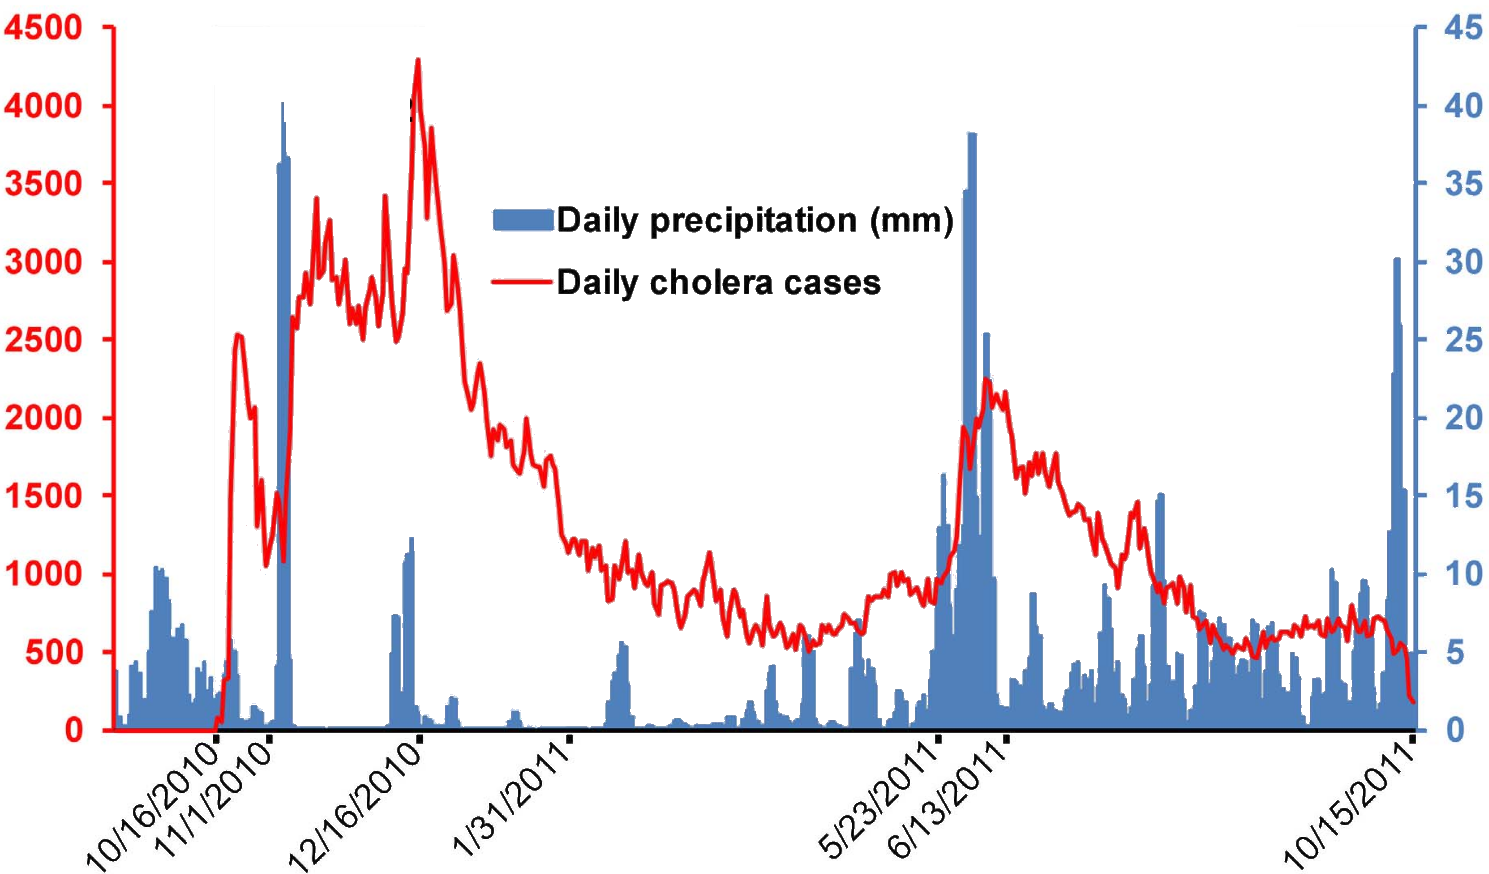
\includegraphics{fig/cholera-rainfall.png}
\margincaption[Similarities between daily cholera incidence and rainfall in Haiti]{\footnotesize Daily cholera cases (red) and daily rainfall (blue) in Haiti from September 15, 2010 to October
16, 2011. It highlights the visual correlation between heavy rainfall event and cholera outbreaks. Adapted from \fullcite{Gaudart:SpatioTemporalDynamicsCholera:2013}.}
\label{fig:rain}
\end{marginfigure}
 Previous studies have highlighted the role of climatic drivers on cholera dynamics, mostly focusing on climate change effects on disease spread\shortcite{Rinaldo:ModelingKeyDrivers:2017,Hashizume:EffectRainfallIncidence:2008,Magny:CholeraOutbreakSenegal:2012,Rodo:ClimateChangeInfectious:2013,Ramirez:NinoClimateCholera:2016,Vezzulli:ClimateInfluenceVibrio:2016} or on the impacts of spatial and temporal heterogeneities\shortcite{Reiner:HighlyLocalizedSensitivity:2012, Baker-Austin:EmergingVibrioRisk:2013, Vezzulli:OceanWarmingSpread:2013, Cash:CholeraShigellosisDifferent:2014,Escobar:GlobalMapSuitability:2015, Vezzulli:EffectsGlobalWarming:2015,Perez-Saez:ClimatedrivenEndemicCholera:2017}. The effect of temperature on cholera transmission has been described (though mainly through the lense of \textit{Vibros} survival and ecology in natural environments), but for rainfall, it remains to be fully elucidated, possibly due to the multiple ways in which it can influence transmission at the local and regional scales\shortcite{Rinaldo:Reassessment20102011:2012,Eisenberg:ExaminingRainfallCholera:2013,Baracchini:SeasonalityCholeraDynamics:2017}. Indeed, intense rainfall events have been shown to alter infection risk through a variety of potential mechanisms, including: flooding, leading to sewage contamination of water sources\shortcite{Ruiz-Moreno:CholeraSeasonalityMadras:2007, Hashizume:EffectRainfallIncidence:2008}; increased hydrologic transport-driven iron availability in environmental waters that enhances pathogen survival and the expression of toxins\shortcite{Lipp:EffectsGlobalClimate:2002,Faruque:SeasonalEpidemicsCholera:2005, Hill:ToxigenicVibrioCholerae:2011}; dry spells inducing persistent low water levels leading to increased use of unsafe water sources\shortcite{Rebaudet:EnvironmentalDeterminantsCholera:2013}; and crowding during strong flood events\shortcite{Reiner:HighlyLocalizedSensitivity:2012}.

Most countries where associations between rainfall and cholera risk have been studied experience endemic cholera transmission. Empirical studies have shown a range of correlations, both positive and negative, endowed with time lags ranging from weeks to months\shortcite{Ruiz-Moreno:CholeraSeasonalityMadras:2007,Emch:SeasonalityCholera1974:2008,Magny:CholeraOutbreakSenegal:2012}. In general, rainfall has been found to increase cholera transmission, but there is evidence of the inverse, possibly due to pathogen dilution\shortcite{Ruiz-Moreno:CholeraSeasonalityMadras:2007}. Such variability reflects the variety of potential mechanisms whereby rainfall may alter infection risk. Similarly, a clear empirical correlation between intense rainfall and enhanced transmission is found in several regions hit by cholera epidemics\shortcite[][but Haiti is treated specifically in the next chapter]{Magny:EnvironmentalSignaturesAssociated:2008,Magny:CholeraOutbreakSenegal:2012,Rebaudet:EnvironmentalDeterminantsCholera:2013,Rebaudet:CholeraCoastalAfrica:2013,Jutla:WaterMarkerMonitored:2013} (fig. \ref{fig:rain}). Results therein showed that at all spatial scales and locations examined, tropical storms were correlated with increased cholera incidence with lags of the order of a few days. As a consequence, accounting for the related forcing of dynamic models resulted in improved fits of reported incidence. 

Properly incorporating the effects of rainfall in mathematical models of cholera transmission is thus paramount to discriminate among the above-mentioned alternative transmission pathways, thus unlocking a predictive framework to evaluate the potentially rainfall-sensitive efficacy of available intervention strategies in endemic and epidemic settings. This becomes  critically important when evaluating the number of averted infections by deploying vaccines, as was done in the aftermath of the passage of Hurricane Matthew\shortcite{Pasetto:RealtimeProjectionsCholera:2017}, or considering optimal deployment in space and time.

The effect of rainfall on indirect cholera transmission has been accounted for in two main fashions in recent mathematical models. On one side, a \textit{contamination}-centered approach suggesting that bursts of infections could be linked to increased contamination of the water compartment\shortcite{Rinaldo:Reassessment20102011:2012}, as in the ECHO model presented in \textsc{Chapter~2}. This process conceptualizes the washout of open-air defecation sites by hydrologic transport. The same `transport' effect may be realized by sewer collectors' overflows. In fact, both mechanisms have the net effect of charging progressively the bacterial concentration in the water reservoir\shortcite{Codeco:EndemicEpidemicDynamics:2001}. Pathogens' loads are washed out from a hydrologic catchment enclosing human settlements and their infective individuals shedding bacteria. Therein, pathogen survival and thus the toxicity of their loads depend on hydrologic residence time distributions\shortcite{Rinaldo:Reassessment20102011:2012,Rinaldo:ModelingKeyDrivers:2017}. Such loads increase as a function of rainfall, which acts as proxy of runoff volumes. The second approach is \textit{exposure}-centered and employs a rainfall-dependent exposure rate subsuming both pathogen availability and the probability of the ingestion of contaminated water during wet spells\shortcite{Eisenberg:ExaminingRainfallCholera:2013}. Although both approaches are physically plausible, they have not been compared directly on the same datasets within a formal statistical framework, which would allow to highlight their respective merits and further recommendations for their use in different settings.

In this chapter, the explanatory power of these different types of rainfall-driven mechanistic models applied to a cholera outbreak in South Sudan is compared. The link between rainfall and cholera during the outbreak recorded in Juba in 2015, when an intra-seasonal peak of cholera cases was recorded possibly in correspondence to intense precipitation events is quantitatively examined. The analysis of the lagged relationship between rainfall rates and revamped cholera incidence is addressed via dynamical compartmental models considered both in deterministic and stochastic versions incorporating both direct (human-to-human) and indirect (water-to-human) disease transmission, and rainfall effects on both contamination and exposure.
\section{Case study: the 2015 cholera outbreak in Juba, South Sudan}\label{sec:data sets}
\begin{figure}\centering
  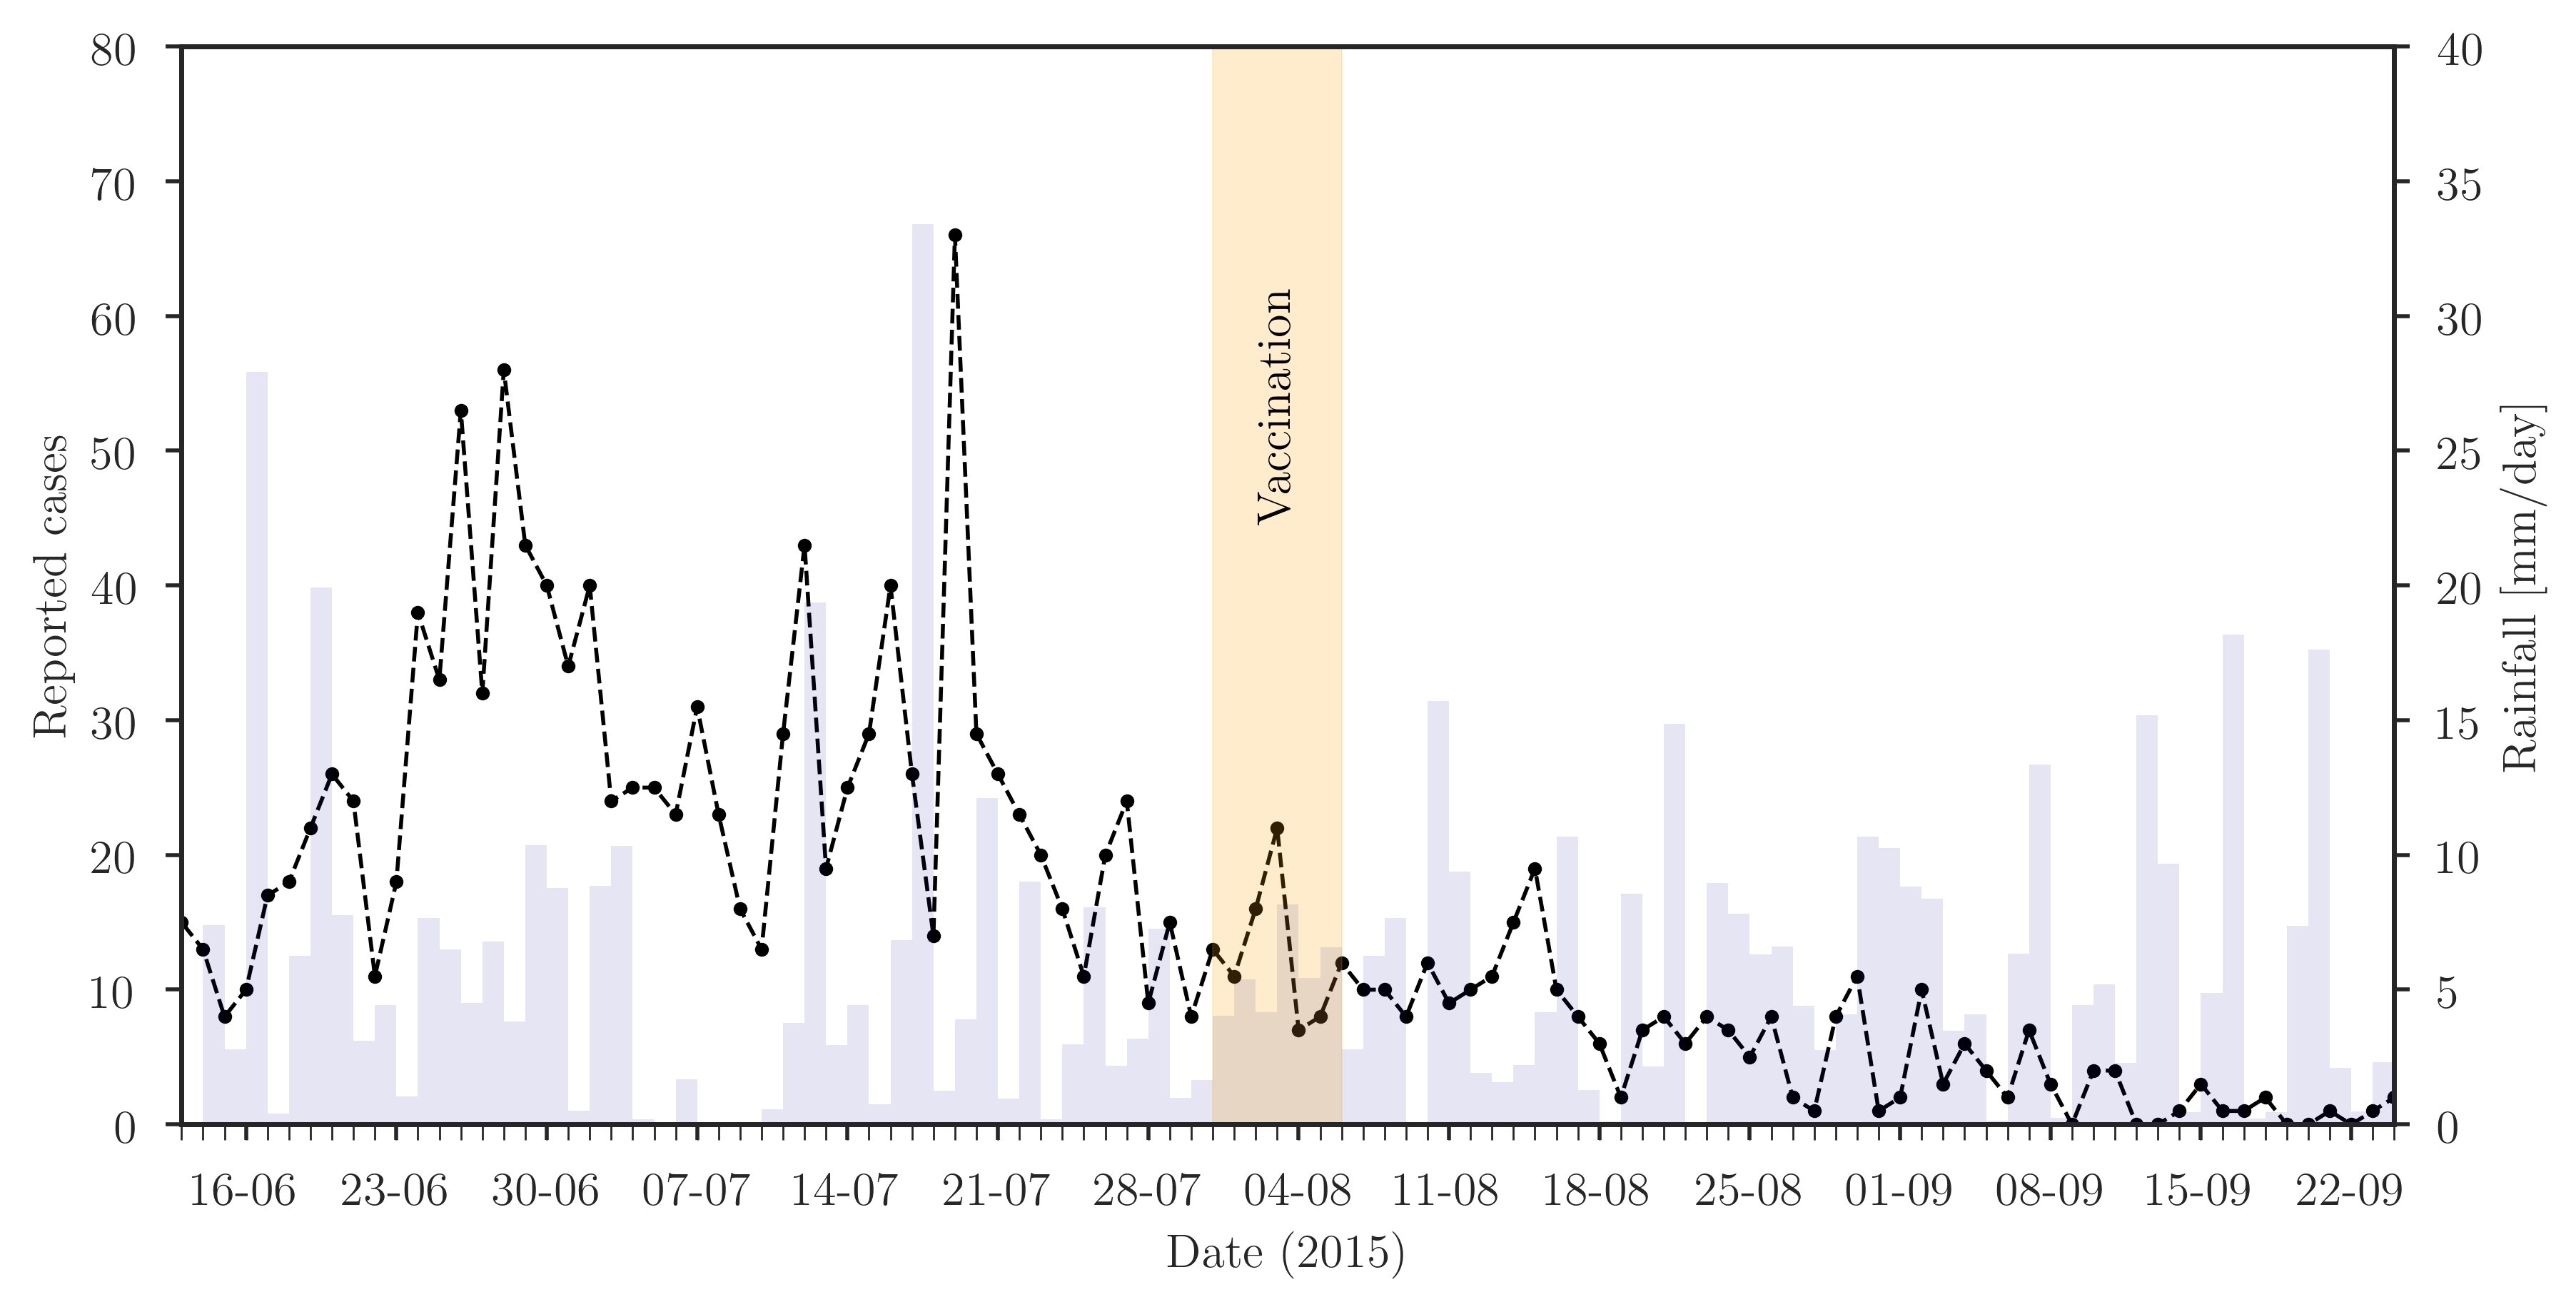
\includegraphics{fig_cholera-rainfall/Lemaitre_ACTROP_2018_42_R1_fig2.png}
  \caption[Cholera cases and precipitation during the 2015 cholera epidemic in Juba][2\baselineskip]{Reported cholera cases (dots) and precipitation (bars) during the 2015 cholera epidemic in Juba. The timing of the vaccination campaign is highlighted in yellow.}\label{fig:report}
\end{figure}
In the past years, South Sudan had been struck by several cholera outbreaks\footnote{More details on the history of cholera in South Sudan are found in: \fullcite{Sciarra:MathematicalModelingCholera:2018}}. Here the analysis focuses on the 2015 outbreak in Juba, when a particular double peak of cholera cases was associated to a strong intra-seasonal precipitation event (fig.~\ref{fig:report}). Access was to granted to epidemiological records for the 2014 and 2015 cholera epidemics that include daily cholera incident cases and hospitalization at the second-lowest administrative level (Payams), reported by the Ministry of Health of South Sudan. The cases in the 7 Payams that constitute the administrative area of Juba have been aggregated to obtain the reported time series for the county level. The population data for Juba county is taken from the South Sudan National Bureau of Statistics\cite[-4\baselineskip]{SSNBS:PopulationProjectionsSouth:2015}. Daily rainfall estimates for years 2014 and 2015 were obtained from the Climate Data Library\cite[-3.5\baselineskip][with a resolution of {0.1}$^\circ$, rainfall was averaged over the study area.]{IRI/LDEO:ClimateDataLibrary:2016}. In 2015, 167'377 OCV doses were distributed in the county of Juba during 6 days of a mass vaccination campaign started on July 31, 2015\cite[-3.2\baselineskip]{Abubakar:FirstUseGlobal:2015,Azman:EffectivenessOneDose:2016,Parker:AdaptingGlobalShortage:2017}, and are taken into account in the model.
%FFN: South Sudan has a lot of one dose
\newpage
\section{Cholera models}
\label{sec:meth}
\subsection{Generalized cholera model}
The proposed model is inspired from the model presented in the previous chapter: we have the susceptible $S$, infected $I$, and recovered $R$ compartments for individuals, with an additional variable $B$ describing the concentration of the bacteria in the environment. Previous modelling exercises had considered rainfall intensity $J(t)$ either to i) multiplicatively increase water \textit{contamination} with bacteria shed by infected  individuals\cite{Bertuzzo:ProbabilityExtinctionHaiti:2016,Pasetto:RealtimeProjectionsCholera:2017}, or ii) assumed that the rainfall multiplicatively increases the \textit{exposure} to contaminated water\cite{Eisenberg:ExaminingRainfallCholera:2013}. A generalized formulation of these cholera-forced models, wherein both formulations are nested, is proposed. It enables the systematic comparison of the effect of rainfall through these two different transmission pathways.

The model described in \textsc{Chapter~1} was designed to deal with weekly data. Here, given the daily temporal resolution at which incidence data was available for the 2015 Juba's epidemic, a compartment of exposed individuals $E$ is added to the model structure. It describe the incubation period: the lag between the time of exposure and the onset of the symptoms. Moreover, in order to account for the vaccination campaigns that were deployed in Juba in August 2015, four compartments ($V^S$, $V^E$, $V^I$, and $V^R$) are added to describe the dynamics of vaccinated individuals and their removal from the pool of susceptibles.

The proposed generalized cholera model is described in fig.~\ref{diagram}, and formulated as:
\marginnote[7\baselineskip]{
\begin{tabular}{ll}
\toprule
     symbol      & signification   \\
    \hline
$\alpha$ & cholera induced mortality\\
$\mu$ & natural mortality\\
$\sigma$ &symptomatic fraction\\
$\gamma$ & infectious period \\
$\rho$ & duration of immunity \\
$\rho_v$ & duration of vaccine protection \\
$\eta$ & vaccine efficacy \\
$\theta$ & shedding rate \\
$\mu_B$ & bacteria decay in water \\
$J(t)$ & rainfall \\
\bottomrule
\end{tabular}\\Reminder of the parameters already described in \textsc{Chapter~1} (p.\pageref{eq:I2}).}

\begingroup
\allowdisplaybreaks
\begin{eqnarray} \label{eq:fullmodel}
S(t) &=& H - I(t) - E(t) - R(t) - V^S(t) - V^E(t) - V^I(t) - V^R(t) \label{eq:S2j} \\
 \frac{dE}{dt} &=& \sigma F(t) S - (\phi + \mu +\nu) E \label{eq:E2j}\\
 \frac{dI}{dt} &=& \phi E - (\gamma + \mu + \alpha) I \label{eq:I2j}\\
 \frac{dR}{dt} &=& (1-\sigma) F(t) S + \gamma I - (\rho + \mu+\nu) R \label{eq:R2j}\\
 \frac{dB}{dt} &=& - \mu_B B +\theta\left[1 + f_{\mathcal{c}}\left(J(t)\right) \right] (I+V^I)\label{eq:B2}\\
\frac{dV^S}{dt} &=& \nu S - \mu V^S+ \rho_{v} V^R - (1-\eta) F(t) V^S \label{eq:VS2j}\\
 \frac{dV^E}{dt} &=& \nu E + \sigma (1-\eta) F(t) V^S-(\phi + \mu) V^E \label{eq:VE2}\\
 \frac{dV^I}{dt} &=&  \phi V^E -(\gamma + \alpha + \mu) V^I \label{eq:VI2j}\\
 \frac{dV^R}{dt} &=& \nu R -(\mu +\rho_{v})V^R +\gamma V^I +(1-\sigma) (1-\eta) F(t) V^S\label{eq:VR2j}\; ,
\end{eqnarray}
\endgroup
where $F(t)$ takes into account both human-to-human transmission and nonlinear water-to-human transmission:
\begin{equation}
  F(t) = \beta_B \underbrace{ \left[\frac{B}{K + B} \right] \bigg(1+f_{\mathcal{e}}\left(J(t)\right)\bigg)}_{\text{indirect transmission}} + ~\beta_{I} \underbrace{\frac{(I+V^I)}{H}}_{\text{direct transmission}}.
\label{eq:force2}
\end{equation}
 The notation is consistent with \textsc{Chapter~1} and we refer the reader to the description of the processes provided on \pageref{eq:I2}, and reminded in the margin table. In addition to tge previously decribed dynamics, exposed individuals become symptomatic infected at a rate $\phi$, which corresponds to an average incubation period of $1/\phi\approx$ 1.5 days\cite{Azman:IncubationPeriodCholera:2013}. As few reliable data on changes in Juba's population are available for the years of interest, the total population $H$, is assumed to be constant, as in \eqref{eq:S2j}. 
 
Moreover, the effect of rainfall is more precisely described. Functions $f_{\mathcal{c}}\left(J(t)\right)$ and $f_{\mathcal{e}}\left(J(t)\right)$ account for the rainfall effect respectively by increasing the bacteria contamination in the water reservoir or directly through amplifying the exposure in the force of infection.
\begin{figure}
  \centering
  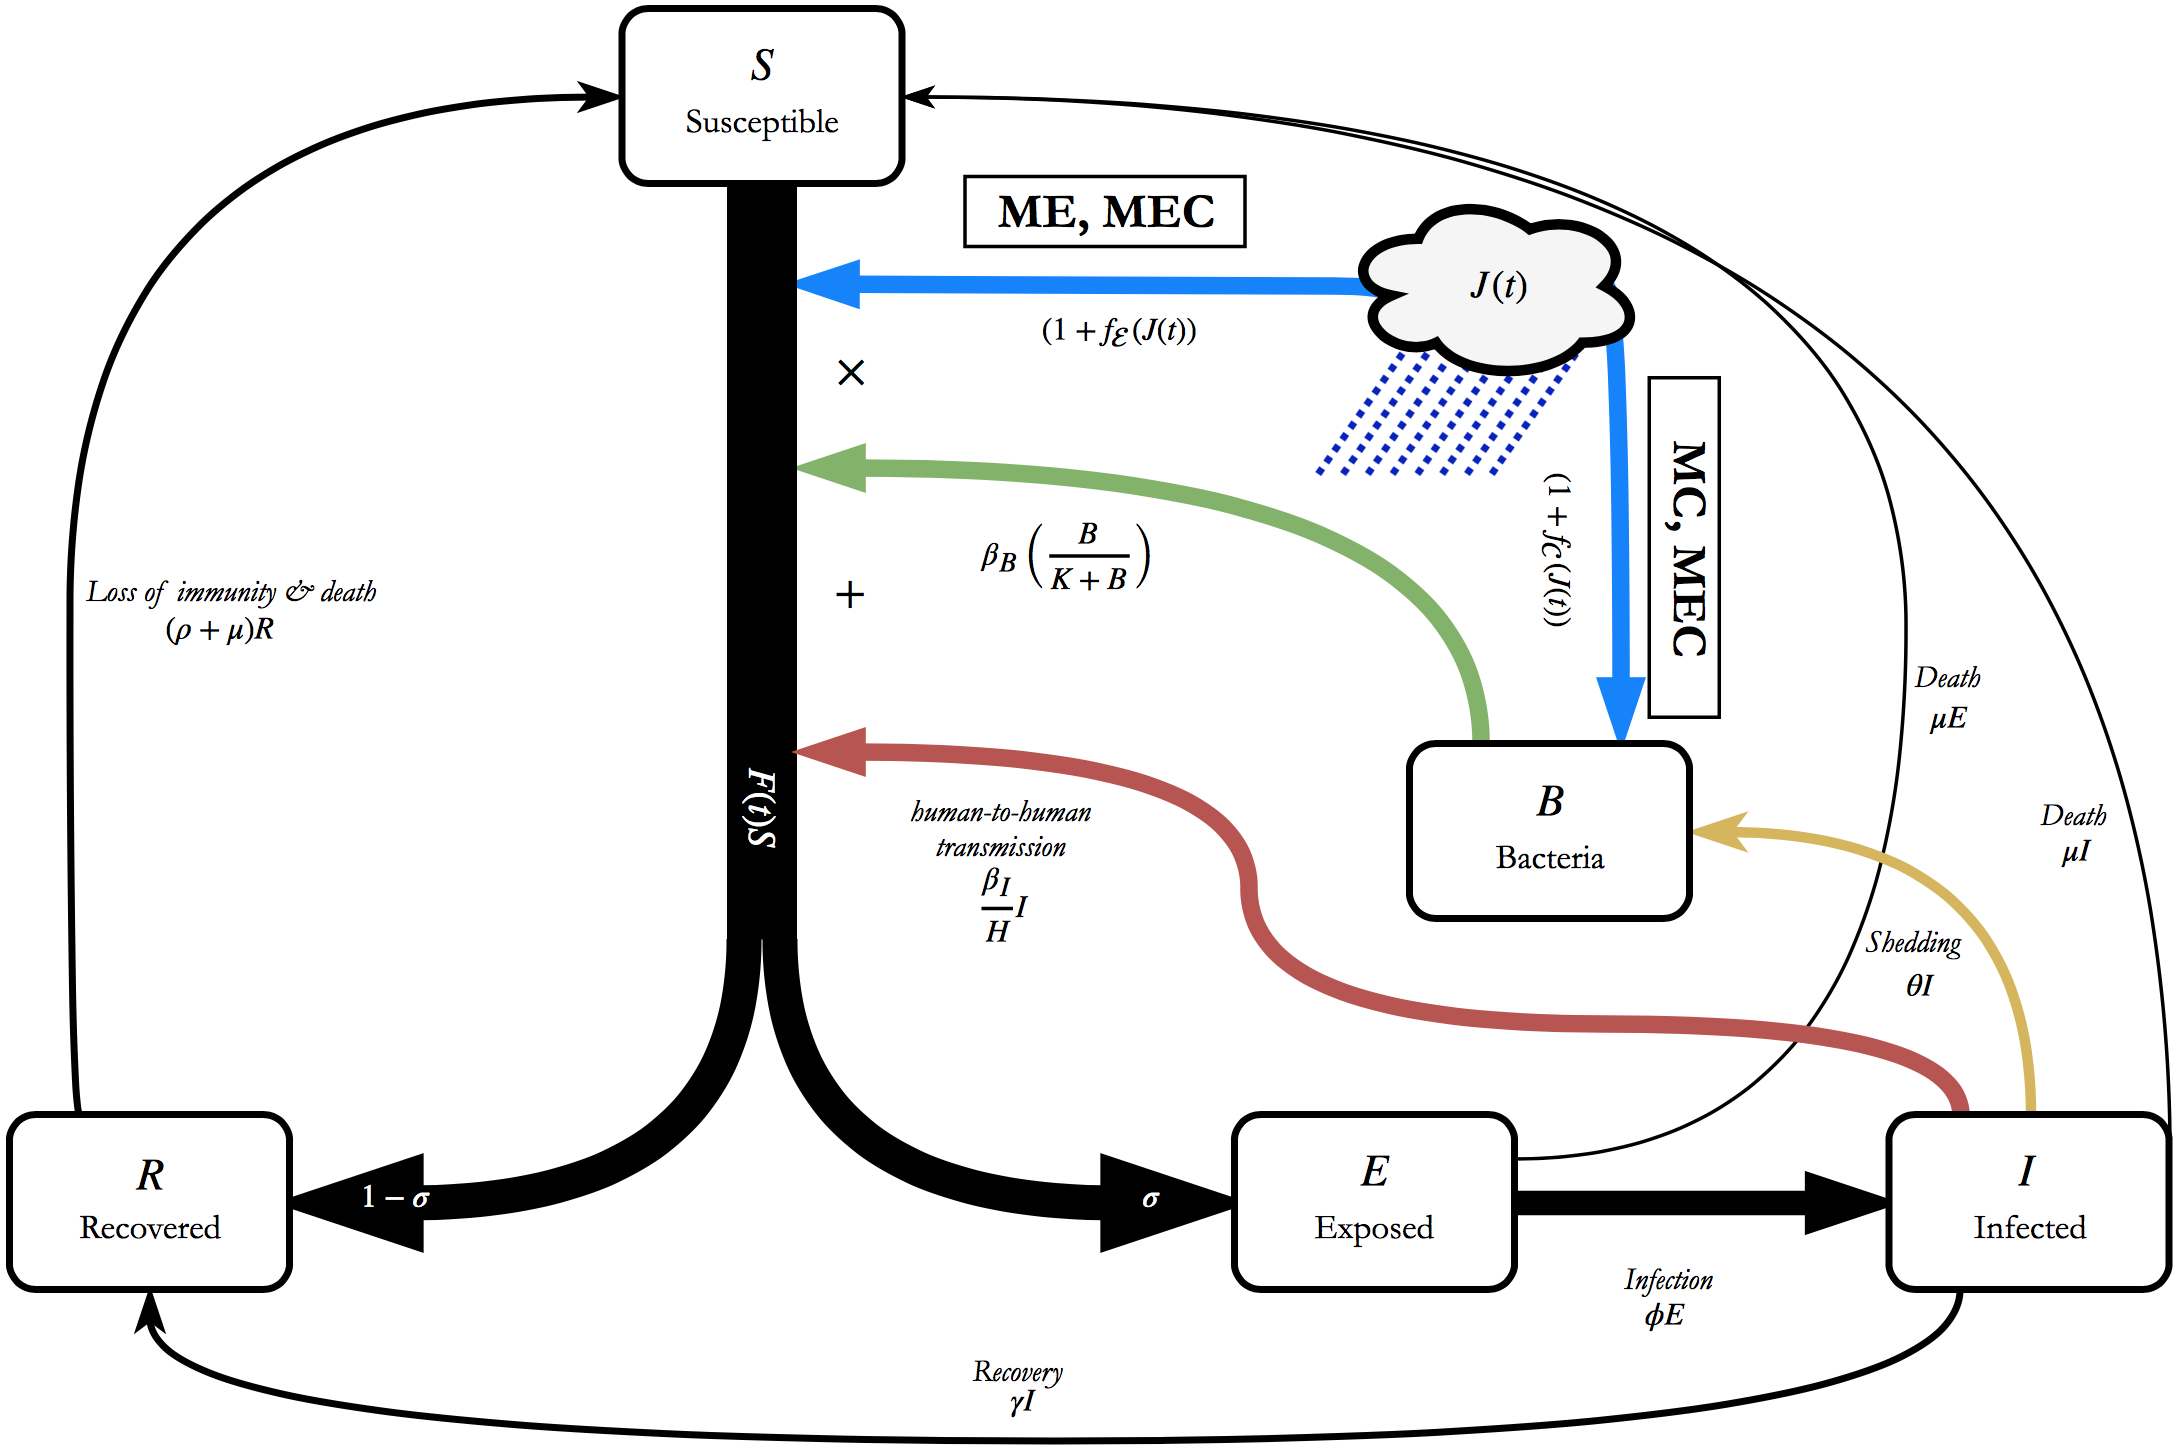
\includegraphics{fig_cholera-rainfall/Lemaitre_ACTROP_2018_42_R1_fig1.png}
  \caption[Transition diagram for the competing cholera models]{Transition diagram for the different cholera models considered, with the different variations \textsc{me}, \textsc{mr}, and \textsc{mec} indicated.}
  \label{diagram}
\end{figure}
With the objective of assessing the importance of rainfall on cholera transmission, a generalization of the linear relation found in the litterature\footnote{Specifically the reference exposure \parencite{Eisenberg:ExaminingRainfallCholera:2013} and contamination \parencite{Rinaldo:Reassessment20102011:2012} models.} is proposed, by using a nonlinear function form for  $f_{\mathcal{c,e}}\left(J(t)\right)$:
\begin{equation}
    f_{\mathcal{c,e}}\left(J(t)\right)=\lambda_{\mathcal{c,e}} \left(\frac{J(t)}{\max_t J(t)}\right)^{\alpha_{\mathcal{c,e}}}
    \label{eq:nonlinear_rain}
\end{equation}
\begin{marginfigure}
	\centering
	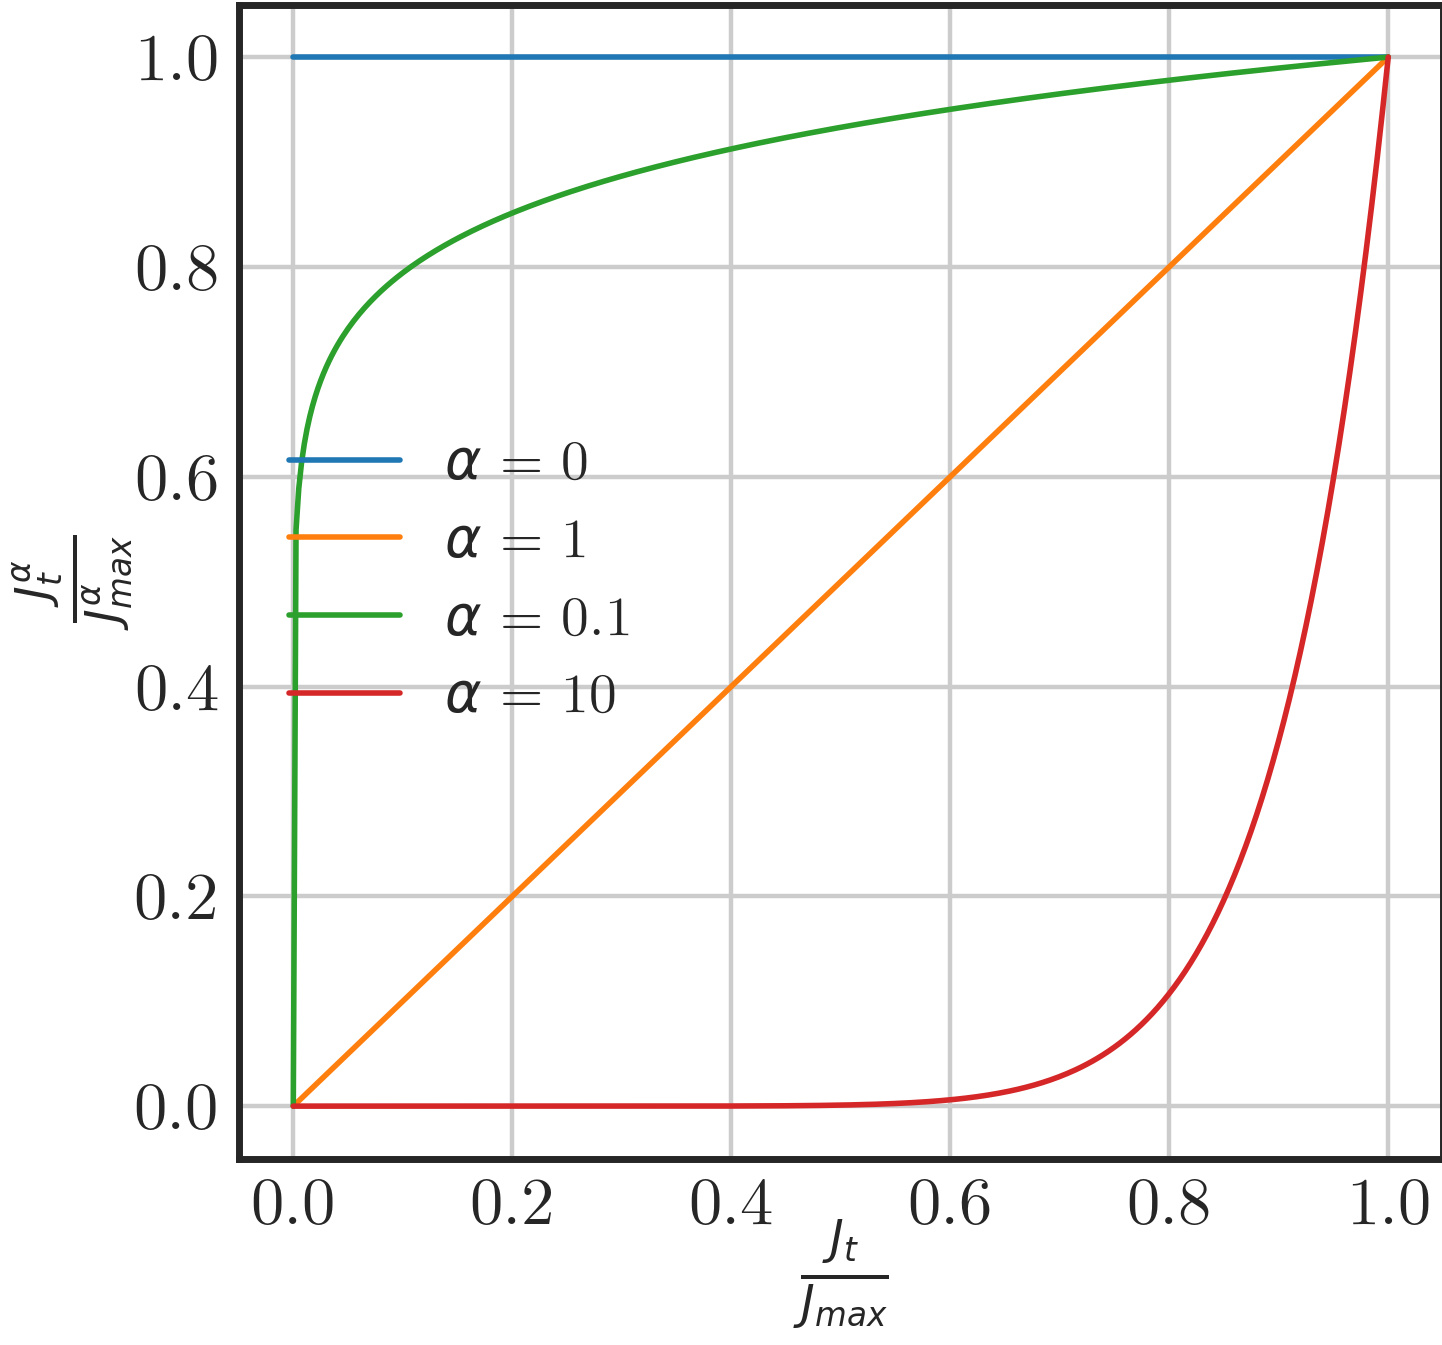
\includegraphics{fig_cholera-rainfall/alpha.png}
	\margincaption[Non-linear rainfall effect on transmission]{$\left(\frac{J_t}{J_{max}}\right)^\alpha$ for different values of $\alpha$. For $\alpha = 1$, the linear model described in previous works is obtained, and larger $\alpha$ corresponds to an increased relative importance of heavy rainfall events.}
	\label{fig:alpha}
\end{marginfigure}
where the subscripts $_\mathcal{c,e}$ respectively denote the effect of rainfall on exposure and contamination, $\max_t J(t)$ is the maximum recorded rainfall intensity during the epidemic, and the $\alpha_{\mathcal{c,e}}\ge0$ controls for the relative importance of different rainfall intensities in their effect on the force of infection. Indeed, since the ratio $\frac{J(t)}{\max_t J(t)} \in [0,1]$, for $\alpha_{\mathcal{c,e}} \gg 1$ the ratio will tend to $0$ for all small precipitation events, leaving only the effect of the strongest events, whereas for $\alpha_{\mathcal{c,e}} < 1$ all precipitation events will be assigned a similar weight in the force of infection (fig. \ref{fig:alpha}). The formulations found in litterature are recovered by setting $\alpha_{\mathcal{c,e}} = 1$. The flexibility allowed by eqn.~\eqref{eq:nonlinear_rain} allows to discriminate between rainfall effects along a continuum from acting on disease transmission regardless of intensity to a threshold-like effect for the largest events which could be associated to severe flooding causing damages to the city's water and sanitary system, for instance leading to sewer overflow.

\subsection{Competing transmission models}
The relevance of the two rainfall-driven transmission pathways is assessed here by comparing the following models:
\begin{itemize}
 \item \textsc{mn} SIRB model without rainfall: $\lambda_{\mathcal{c}} = \lambda_{\mathcal{e}} = 0$, $\beta_{I} = 0$, as the null hypothesis for the importance of rainfall.
  \item \textsc{mc} SIRB model where for rainfall enhances the \textit{contamination} of the water reservoir: $\lambda_{\mathcal{e}} = 0$, $\beta_{I} = 0$. 
  \item \textsc{me} SIRB model where rainfall increases the \textit{exposure} to bacteria: $\lambda_{\mathcal{c}} = 0$, $\beta_{I} = 0$. 
  \item \textsc{mec} SIRB model combining both approaches \textsc{mc} and \textsc{me} ($\beta_{I} = 0$). Both ways of accounting rainfall play a role simultaneously.
\end{itemize}
\marginnote[-8\baselineskip]{\textsc{me} models uses a similar transmission pathway as in \textcite{Eisenberg:ExaminingRainfallCholera:2013}, whereas \textsc{mc} models were described in \textcite{Rinaldo:Reassessment20102011:2012}. These models were adapted to the generalized configuration, \eg in eqn.~\eqref{eq:force2} precipitation enters in the term $\left(1+f_E \left(J(t)\right)\right)$ which entails water-to-human transmission also when $J(t)=0$, unlike the published version. The steps take to adapt these models are shown in the postprint supplementary, section S.1.}
\begin{table}[h!]
\centering
\begin{tabular}{lccccc}
\toprule
     Model       & $\lambda_{\mathcal{c}}$ & $\alpha_\mathcal{c}$ & $\lambda_{\mathcal{e}}$ & $\alpha_\mathcal{e}$ & $\beta_I$   \\
    \hline
    \textsc{mn} &       --    &    --   &       --      &       --      &  -- \\
    \textsc{mnh} &     --      &   --    &    --         &        --     &   $\times$ \\
    \textsc{mc} &      $\times$  &  $\times$  &     --        &       --      &  -- \\
    \textsc{me} &         --  &   --    &      $\times$    &   $\times$        & --  \\
    \textsc{mch}&      $\times$  &  $\times$  &      --       &     --        &$\times$ \\
    \textsc{meh}&        --   &  --     &      $\times$    &   $\times$        &$\times$ \\
    \textsc{mec}&      $\times$ &  $\times$  &      $\times$    &    $\times$      & --\\
    \textsc{mech}&      $\times$ &  $\times$  &      $\times$    &    $\times$       &   $\times$ \\
\bottomrule
\end{tabular}
\caption[Parameters considered in the eight compared models]{Parameters considered in the eight compared models.  $\lambda$ and $\alpha$ characterize the functional forms considering the precipitation eqn.~\eqref{eq:nonlinear_rain}. $\beta_I$ is the exposure for human-to-human transmission. A dash -- indicate that the parameter is set to zero, whereas a cross $\times$  indicate that the parameter is used.}
\label{tab:models}
\end{table}

 For each model is explored the possibility of adding explicitly direct, human-to-human transmission ($\beta_{I} > 0$), which is indicated with an \textsc{H} at the end of the model name: \textsc{mnh}, \textsc{mch}, \textsc{meh}, and \textsc{mech}. The different parameters associated with the considered models are summarized in tab.~\ref{tab:models}.

 The eight models are compared on the basis of their ability to match the time series of daily reported cases during the cholera epidemic in Juba of 2015. In the postprint, tab. S.1 summarizes which parameters are calibrated for each model and their prior distribution. The degrees of freedom of the models, $n_p$, vary from $n_p=7$ for \textsc{mn} to $n_p=12$ for \textsc{mech}. Given the low number of daily reported cases and their ensuing variability, a stochastic equivalent is also implemented\footnote[][-8\baselineskip]{The sole difference in formulation is the introduction of overdispersion in the infection process. The force of infection is multiplied by a time-continuous white noise process, as detailled in the eqns. \eqref{eqn:sta}--\eqref{eqn:stb}.} of the deterministic ODE system, eqns. \eqref{eq:fullmodel}-\eqref{eq:VR2j}, formulated as a continuous time partially observed Markov process model, accounting for both demographic and disease transmission stochasticities\cite{Breto:TimeSeriesAnalysis:2009}. The formulation of the stochastic model is left in the \textsc{Appendix}, eqn. \eqref{eq:stochsys} on p. \pageref{eq:stochsys}.

\subsection{Models calibration}
\marginnote{For details about fixed and calibrated parameters, along with prior and posterior distributions, the reader is referred to the supplemental information of \fullcite{Lemaitre:RainfallDriverEpidemic:2019}.}
\paragraph{Initial conditions} The past history of cholera epidemics in South Sudan, and particularly in Juba, plays an important role in the determination of the size of susceptible and recovered compartments at the beginning of the 2015 epidemic. These two compartments are also largely impacted by the rate of immunity loss $\rho$ of the recovered individuals, and by the probability of asymptomatic infection $1-\sigma$\footnote[][2\baselineskip]{values in literature range between $\sigma=0.5$, meaning one asymptomatic per each symptomatic infected, to less than $\sigma=0.01$, corresponding to more than 99 asymptomatic infected per each symptomatic infected \parencite{Fung:CholeraTransmissionDynamic:2014}.}. The initial conditions must therefore be estimated for each parameter set considered during calibration.

 
 To take into account the uncertainty associated with the immunity landscape of Juba, the initial number of recovered individuals in April 2014 is calibrated for each model. Then, the detailed daily data of suspected cases during 2014 is used to estimate the associated number of recovered individuals at the start of the 2015 epidemic. Suspected cases in 2014 are scaled to the reporting fraction and  undergo an exponential decay with average time of immunity loss $1/\rho$\footnote{Something similar has been done in \parencite{Pasetto:RealtimeProjectionsCholera:2017}.}. Simulations are then initialized on June 5, 2015 considering two exposed individuals, two infected, and the associated steady-state bacteria concentration. 
 
\paragraph{Calibration} Calibration of the deterministic model is performed using a Markov Chain Monte Carlo based algorithm\footnote{Differential Evolution Adaptive Metropolis, \textsc{dream}: \parencite{Vrugt:MarkovChainMonte:2016}, which was developed to explore high-dimensional parameter spaces. Given the parameters' prior distribution, \textsc{dream} searches and selects new samples in the posterior distribution by using multiple \textsc{mcmc} chains that run in parallel and that jointly contribute to the computation of the proposal parameter samples. \textsc{Mcmc} chains  converge toward the posterior probability distribution based on the log-likelihood function of the data given the model output.} , which draws samples from the posterior distribution of the parameters.
Inference on the stochastic model is performed using a frequentist iterated filtering algorithm\footnote{MIF, an algorithm proposed by \parencite{Ionides:InferenceDynamicLatent:2015}, which is a frequentist-based approach for identifying the maximum likelihood estimation. It has proved successful even for a range of complex models of cholera dynamics \parencite{King:InapparentInfectionsCholera:2008,Baracchini:SeasonalityCholeraDynamics:2017}. The MIF2 algorithm, which employs iterated Bayes maps, is implemented in the R package \texttt{pomp} \parencite{King:StatisticalInferencePartially:2015}. %For this exercise, it is configured using 120 initial parameter vectors for each model, built using Sobol sequences over the parameter bounds.
}. Both model were fit against the daily reported cases accounting for over- or under- reporting, and assuming a Poisson likelyhood\shortcite{Camacho:CholeraEpidemicYemen:2018}. Each datapoint at reporting date $t_i$,  $y_{t_i}$, is assumed to belong to a Poisson distribution centered on the modeled incidence $C_{t_i}$\footnote{$C_{t_i}$ is computed as in  eqn. \eqref{eq:C}, but for the $E \rightarrow I$ transition. For the deterministic model: $ C_{t_i} = \int_{t_i}^{t_{i+1}} \phi \left(E(t) + V^E(t)\right) dt$. For the stochastic model the reporting process is described in eqn. \eqref{eq:stochrep}.
% $ C_{t_i} = [N_{EI}(t_{i+1}) - N_{EI}(t_i)] + [N_{V^EV^I}(t_{i+1}) - N_{V^EV^I}(t_i)] $, where $N_{AB}$ denotes the stochastic counting process of transitions between classes $A$ and $B$ .
} and its associated parameter vector $\boldsymbol{\theta}$ altered by the reporting rate $\epsilon$, as:
\begin{equation}
 y_{t_i}  \sim \text{Poisson}\left(\epsilon \,C_{t_i}(\boldsymbol{\theta})\right), \; \epsilon > 0,
 \label{eq:obs}
\end{equation}
 Models were then compared using the Bayesian Information criterion (BIC), Bayes factors, and the likelihood ratio test for the nested models.
 
 
\section{Results}

\subsection{Model selection of the rainfall effects on cholera transmission}
The summary statistics of the deterministic and stochastic models considered in the study are given in tab.~\ref{tab:stats}. Overall, the stochastic models outperform their deterministic counterparts for all model structures by $\approx 40$ log-likelihood units. Both model types agree in the significance of rainfall in explaining the time series of daily reported cases, in particular through the increased exposure pathway, although the specific ordering of the models differs between model types. The BFs for the deterministic models suggest a strong support for model \textsc{mec}, followed by model \textsc{me} ($BF^{-1}_{ME,MEH} = 0.16$), with very little support for all other models ($BF^{-1}_{\boldsymbol{\cdot},MEH}< 10^{-2}$ for all other models than ME). For the stochastic model, the BFs estimated with the BIC suggest the strongest support for model \textsc{me}, with the basic SIRB model coming in second with 5 times less evidence ($BF^{-1}_{MN,ME} \approx 0.15$). 
\begin{table}[h!]
\centering
\small
\begin{tabular}{lcccccccc}
  \toprule
  & \multicolumn{4}{c}{Deterministic} & \multicolumn{4}{c}{Stochastic} \\
    \cmidrule(rl){2-5}\cmidrule(rl){6-9}
  Model & $n$ & $\hat{\ell}$ & BIC & ${BF}^{-1}$ & $n$ & \makecell{$\hat{\ell}$ \vspace{-.1cm} \\ \scriptsize{(s.e.)}}  & BIC  & $BF^{-1}$ \\ 
  \cmidrule(rl){2-5}\cmidrule(rl){6-9}
  \textsc{mn} &   7 & -368.62 & 770.27 & 3.1E-05 &   8 & \makecell{-326.45 \vspace{-.1cm} \\ \scriptsize{(0.105)}} & 690.65 & 1.5E-01 \\ 
   \textsc{mnh} &   8 & -368.95 & 775.64 & 1.1E-09 &   9 & \makecell{-327.52\vspace{-.1cm} \\ \scriptsize{(0.052)}} & 697.51 & 4.7E-03 \\ 
   \textsc{mc} &   9 & -358.32 & 759.11 & 5.5E-03 &  10 & \makecell{-323.50\vspace{-.1cm} \\ \scriptsize{(0.037)}} & 696.01 & 2.5E-02 \\ 
   \textsc{mch} &  10 & -359.06 & 765.30 & 1.7E-04 &  11 & \makecell{-324.89\vspace{-.1cm} \\ \scriptsize{(0.041)}} & 701.68 & 5.9E-04 \\ 
   \textsc{me} &   9 & -356.96 & \textsc{756.40} & 1.6E-01 &  10 & \makecell{\textsc{-319.81}\vspace{-.1cm} \\ \scriptsize{(0.035)}} & \textsc{687.38} & \textsc{1} \\ 
   \textsc{meh} &  10 & -358.06 & 763.30 & 6.3E-04 &  11 & \makecell{-320.64\vspace{-.1cm} \\ \scriptsize{(0.030)}} & 693.18 & 4.1E-02 \\ 
   \textsc{mec} &  11 & \textsc{-356.87} & 765.64 & \textsc{1} &  12 & \makecell{-320.17\vspace{-.1cm} \\ \scriptsize{(0.031)}} & 696.96 & 6.2E-03 \\ 
   \textsc{mech} &  12 & -357.55 & 771.73 & 2.4E-06 &  13 & \makecell{-320.38\vspace{-.1cm} \\ \scriptsize{(0.024)}} & 702.09 & 4.8E-04 \\ 
   \bottomrule
\end{tabular}
\caption[Model comparison statistics]{Model comparison statistics. For each model is reported its number of parameters $n$, the associated estimated log-likelihood $\hat{\ell}$ (and its Monte Carlo standard error for the stochastic model), and the inverse of the Bayes Factor ($BF^{-1}$) with respect to the model with the largest evidence. The BFs for the deterministic models were computed directly from the parameters posteriors, whereas for the stochastic models they were estimated with the Bayesian Information Criterion (BIC) as $BF_{i} \approx e^{\frac{1}{2} \left( BIC_i - BIC_{min}\right)}$. The BIC for the deterministic models was computed using the maximum log-likelihood value visited with the MCMC algorithm across chains.}\label{tab:stats}
\end{table}
When considering only the BIC, model \textsc{me} ranks first for both the deterministic and the stochastic formulations. Interestingly, all models that include human-to-human transmission present smaller or equal log-likelihoods than their counterparts with only the bacteria compartment, which suggests that the data does not support both environmental and human-to-human transmission within the set of the models considered here.

The results of the nested LR-tests confirm the statistical significance of including rainfall in the cholera transmission models, with the effect on exposure better supported by the data in both model types than the effect on contamination. In the deterministic case, the extension of the basic SIRB (model \textsc{mn}) with rainfall effects were significant for all direct comparisons (fig.~\ref{fig:lltests},\textsc{a}). The addition of human-to-human transmission was not significant mostly due to the above-mentioned lower estimate of the log-likelihood in these models. When considering only a single effect of rainfall (either increasing exposure or contamination), \textsc{me} outperforms \textsc{mc} in terms of likelihood for the same number of parameters. Interestingly, the inclusion of rainfall-induced contamination in model \textsc{me} is rejected due to the very limited increase of the estimated log-likelihood of \textsc{mec}, in contrast with the BFs favouring the latter. Model \textsc{me} is thus the one retained by the LR-tests in the deterministic set of models. In the case of the stochastic models, the LR-tests also highlight the importance of the effect of rainfall on exposure rather than on contamination (fig.~\ref{fig:lltests},\textsc{b}). In fact, the much stronger performance of \textsc{mn} in comparison with its deterministic counterpart relative to all other model structures imposes a stronger condition for retaining additional transmission processes. Indeed, both models \textsc{mc} and \textsc{mch} were rejected when compared to \textsc{mn}, thus only models with rainfall-driven exposure were retained. As in the deterministic case, model \textsc{me} is the one finally retained due to the lack of significance of the inclusion of additional transmission processes. Note that the conclusion based on the LR-tests for the deterministic models should be taken with caution because the \textsc{mcmc} algorithm used for calibration does not directly aim at maximizing the likelihood, but rather at sampling from the posterior distribution of the parameters given the data and the model. Moreover, the best likelihood visited by the chains when sampling the posteriors that are used in the LR-tests is not a formal estimate of the models' likelihood. However, the fact that the LR-tests applied to both model types agree with the selection of \textsc{me} supports their use in both cases.
\begin{figure*}
    \centering
    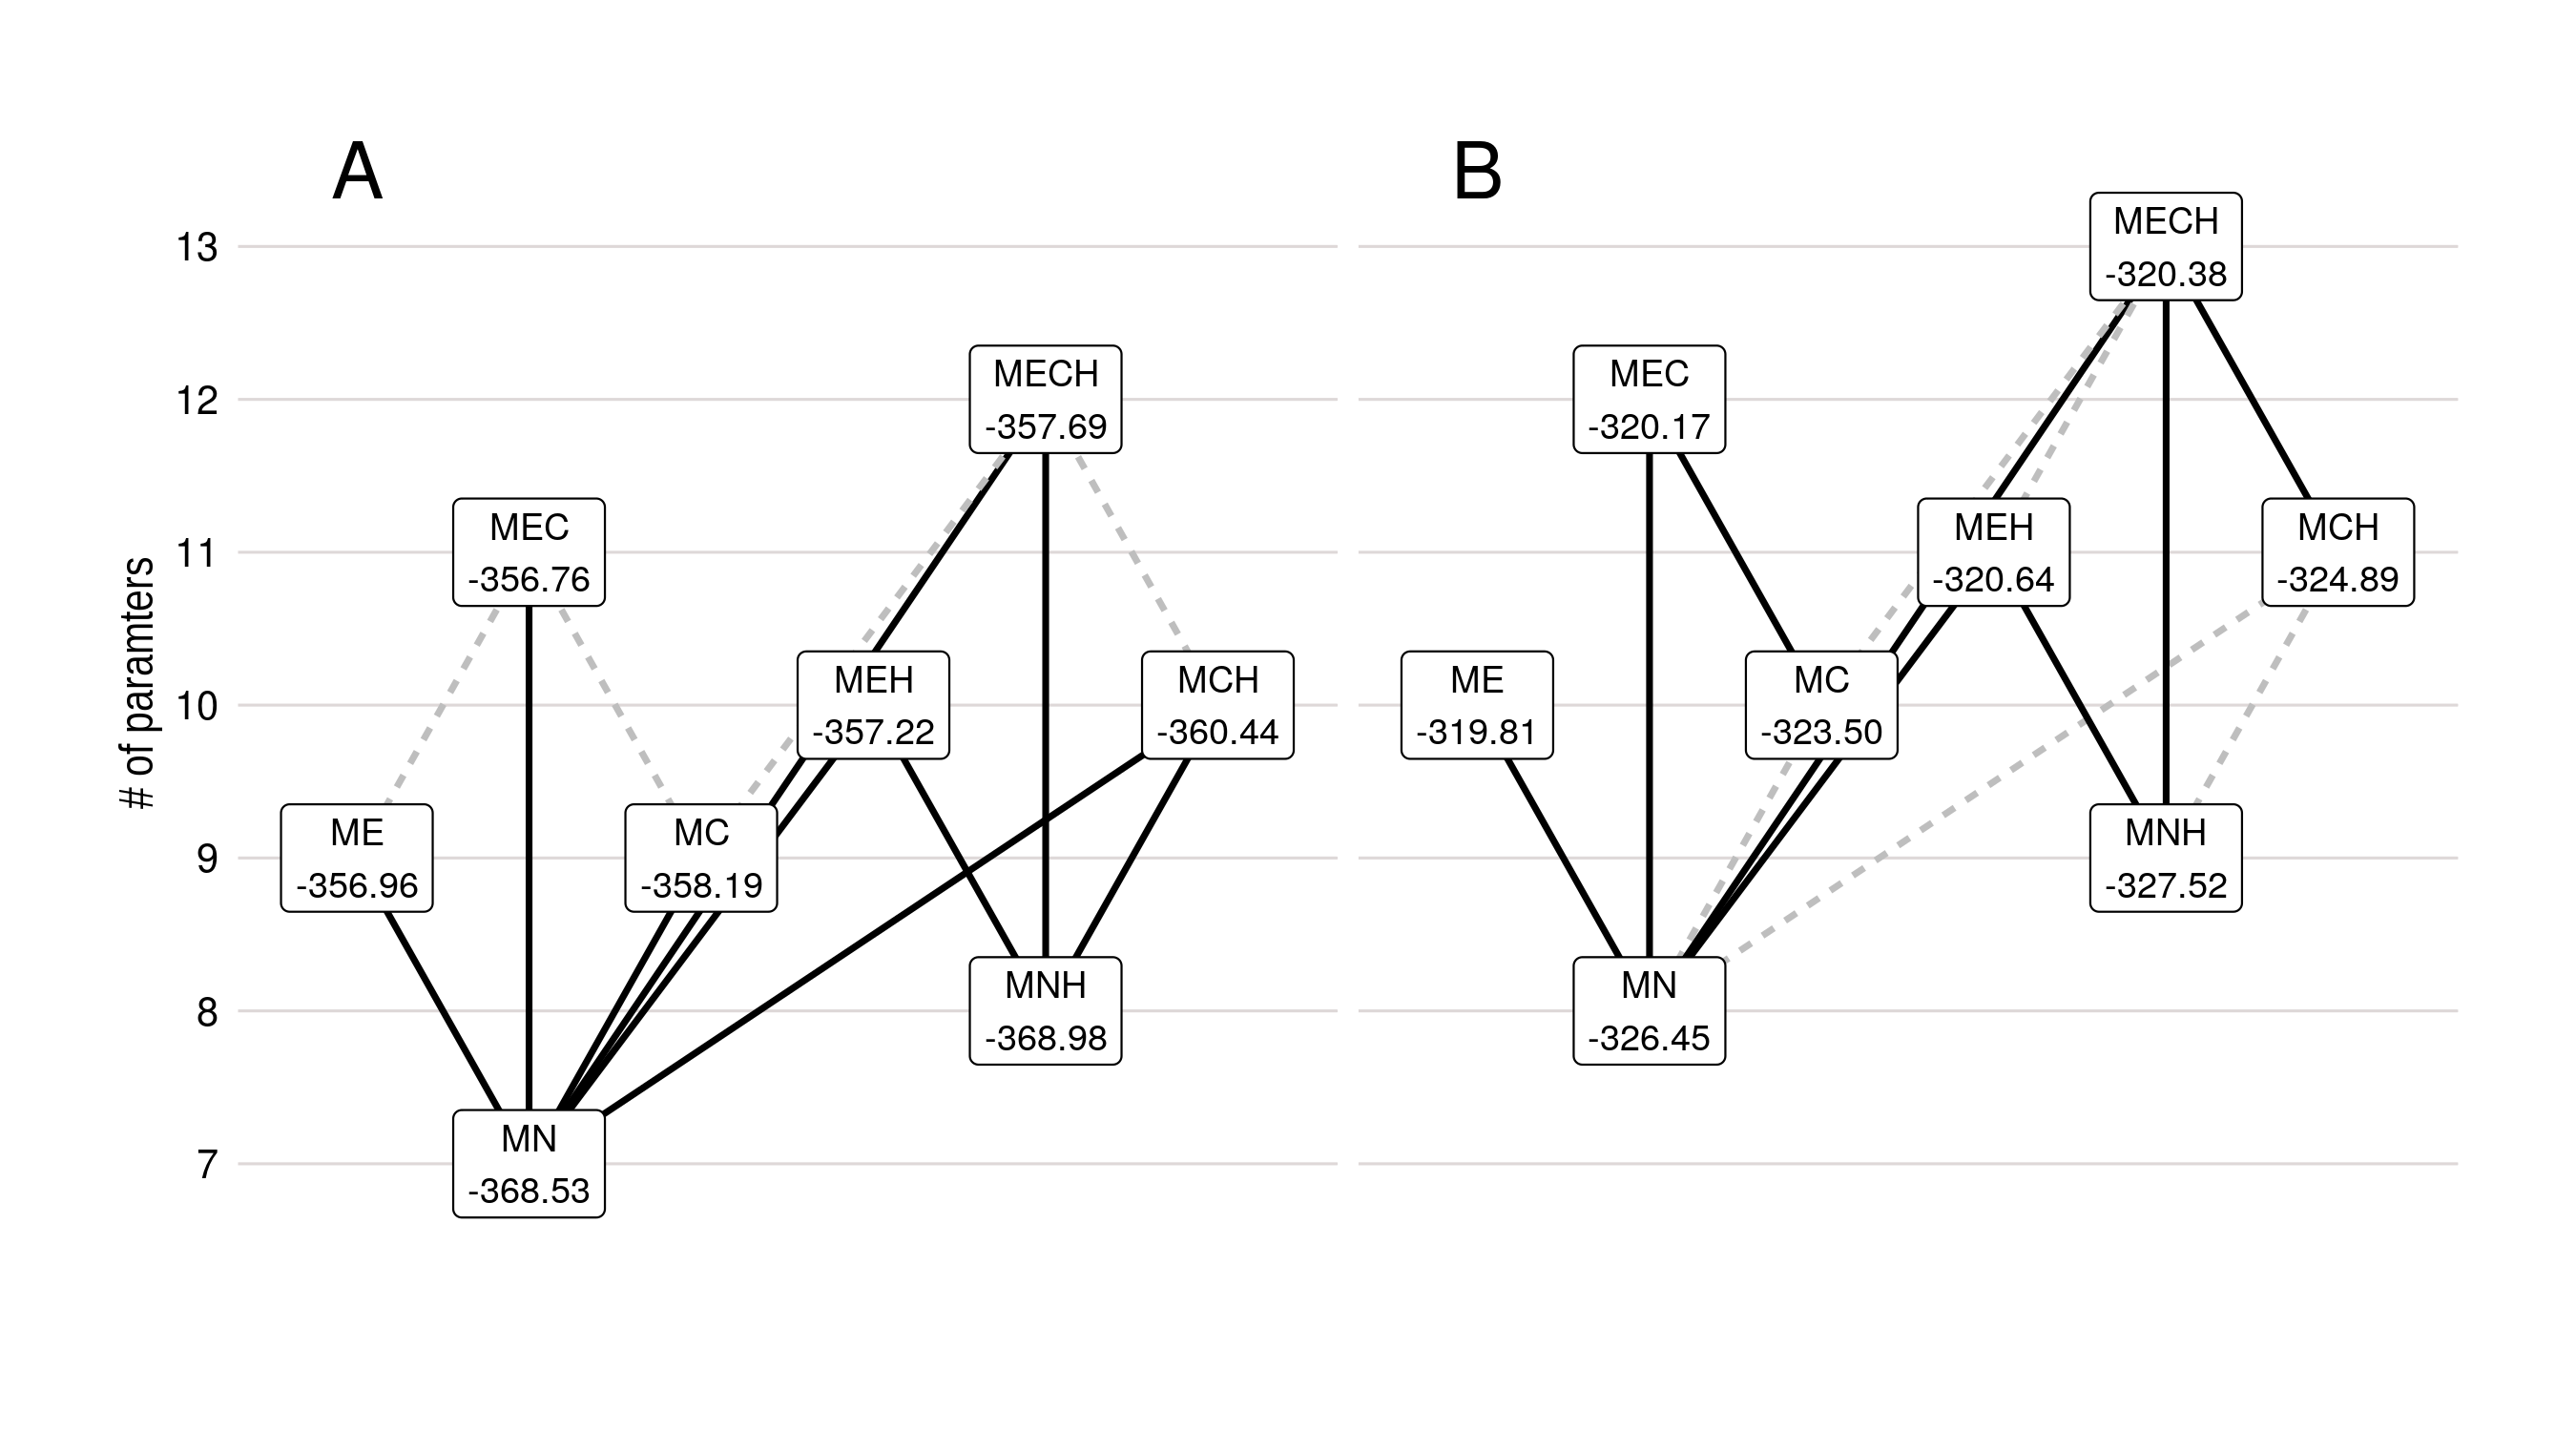
\includegraphics[width = \textwidth, trim = 11mm 19mm 10mm 12mm, clip]{fig_cholera-rainfall/Lemaitre_ACTROP_2018_42_R1_fig3.png}
    \caption[Likelihood ratio tests of model nesting]{Likelihood ratio tests of model nesting. The LL-tests were computed for each nested pair of models $\{\mathcal{M}_0, \mathcal{M}_1\}$, with parameter vectors $\boldsymbol{\theta}^0,\boldsymbol{\theta}^1$, for which at least on of the parameters that is not null is $\boldsymbol{\theta}^1$ is equal to $0$ in $\boldsymbol{\theta}^0$. Each model is labeled with its associated estimated maximum log-likelihood value, $\hat{\ell}$, for the deterministic (A) and the stochastic (B) models, and linked based on whether the likelihood ratio is significantly (full black lines) or not (dashed gray lines) at the 5\% level. The absence of lines indicates a lower $\hat{\ell}$ for the more complex model.} 
    \label{fig:lltests}
\end{figure*}


Both statistical methods for model comparison therefore agree about the importance of the effect of intra-seasonal rainfall on the exposure to transmission during the 2015 cholera epidemic in Juba. For the deterministic type of models the BFs suggest a stronger support for model \textsc{mec}, and the LR-tests for \textsc{me}, whereas for the stochastic models both the BIC-based estimates of BFs and the LR-tests favor \textsc{me}. 

\subsection{Intra-seasonal rainfall events and the 2015 Juba epidemic}

The comparison between the estimated output cases computed by the basic SIRB model (\textsc{mn}) and the most significant rainfall-based processes (\textsc{mec} and \textsc{me} for the deterministic and stochastic types, respectively) highlight the importance of rainfall in retrieving the second epidemiological peak (fig.~\ref{fig:sim}). Both deterministic and stochastic models fit well the general trend of the data, but they clearly underestimate the large number of reported cases on the 19th of July (65 cases). Instead, the more complex models \textsc{me} and \textsc{mec} follow the SIRB dynamics and then are forced by the precipitation occurred in the 18th of July (33 mm/d)  toward the epidemiological peak. 
%

Model calibration results suggest that precipitations with smaller intensities did not have a strong impact on cholera transmission during the 2015 epidemic in Juba. Indeed, the exponents $\alpha_{\mathcal{c}}$ and $\alpha_{\mathcal{e}}$ were found to be systematically larger than 1. %  (as shown by posteriors of the deterministic models in fig. S.2 and the Monte Carlo confidence intervals for the stochastic \textsc{me} in fig. S.4 of the SI) --> appendix or not ? DECISION
  Thus, in the considered epidemic, the nonlinear function used to account for rainfall in the model, eqn.~\eqref{eq:nonlinear_rain}, helps isolating the contribution of the largest rainfall.

The best measures of fit computed for the stochastic \textsc{me} (see tab.~\ref{tab:stats}) are thus explained by a larger sensitivity to precipitation, which causes the match between the mean of the simulated cases and the data during the second peak.

\begin{figure}[ht]
    \centering
    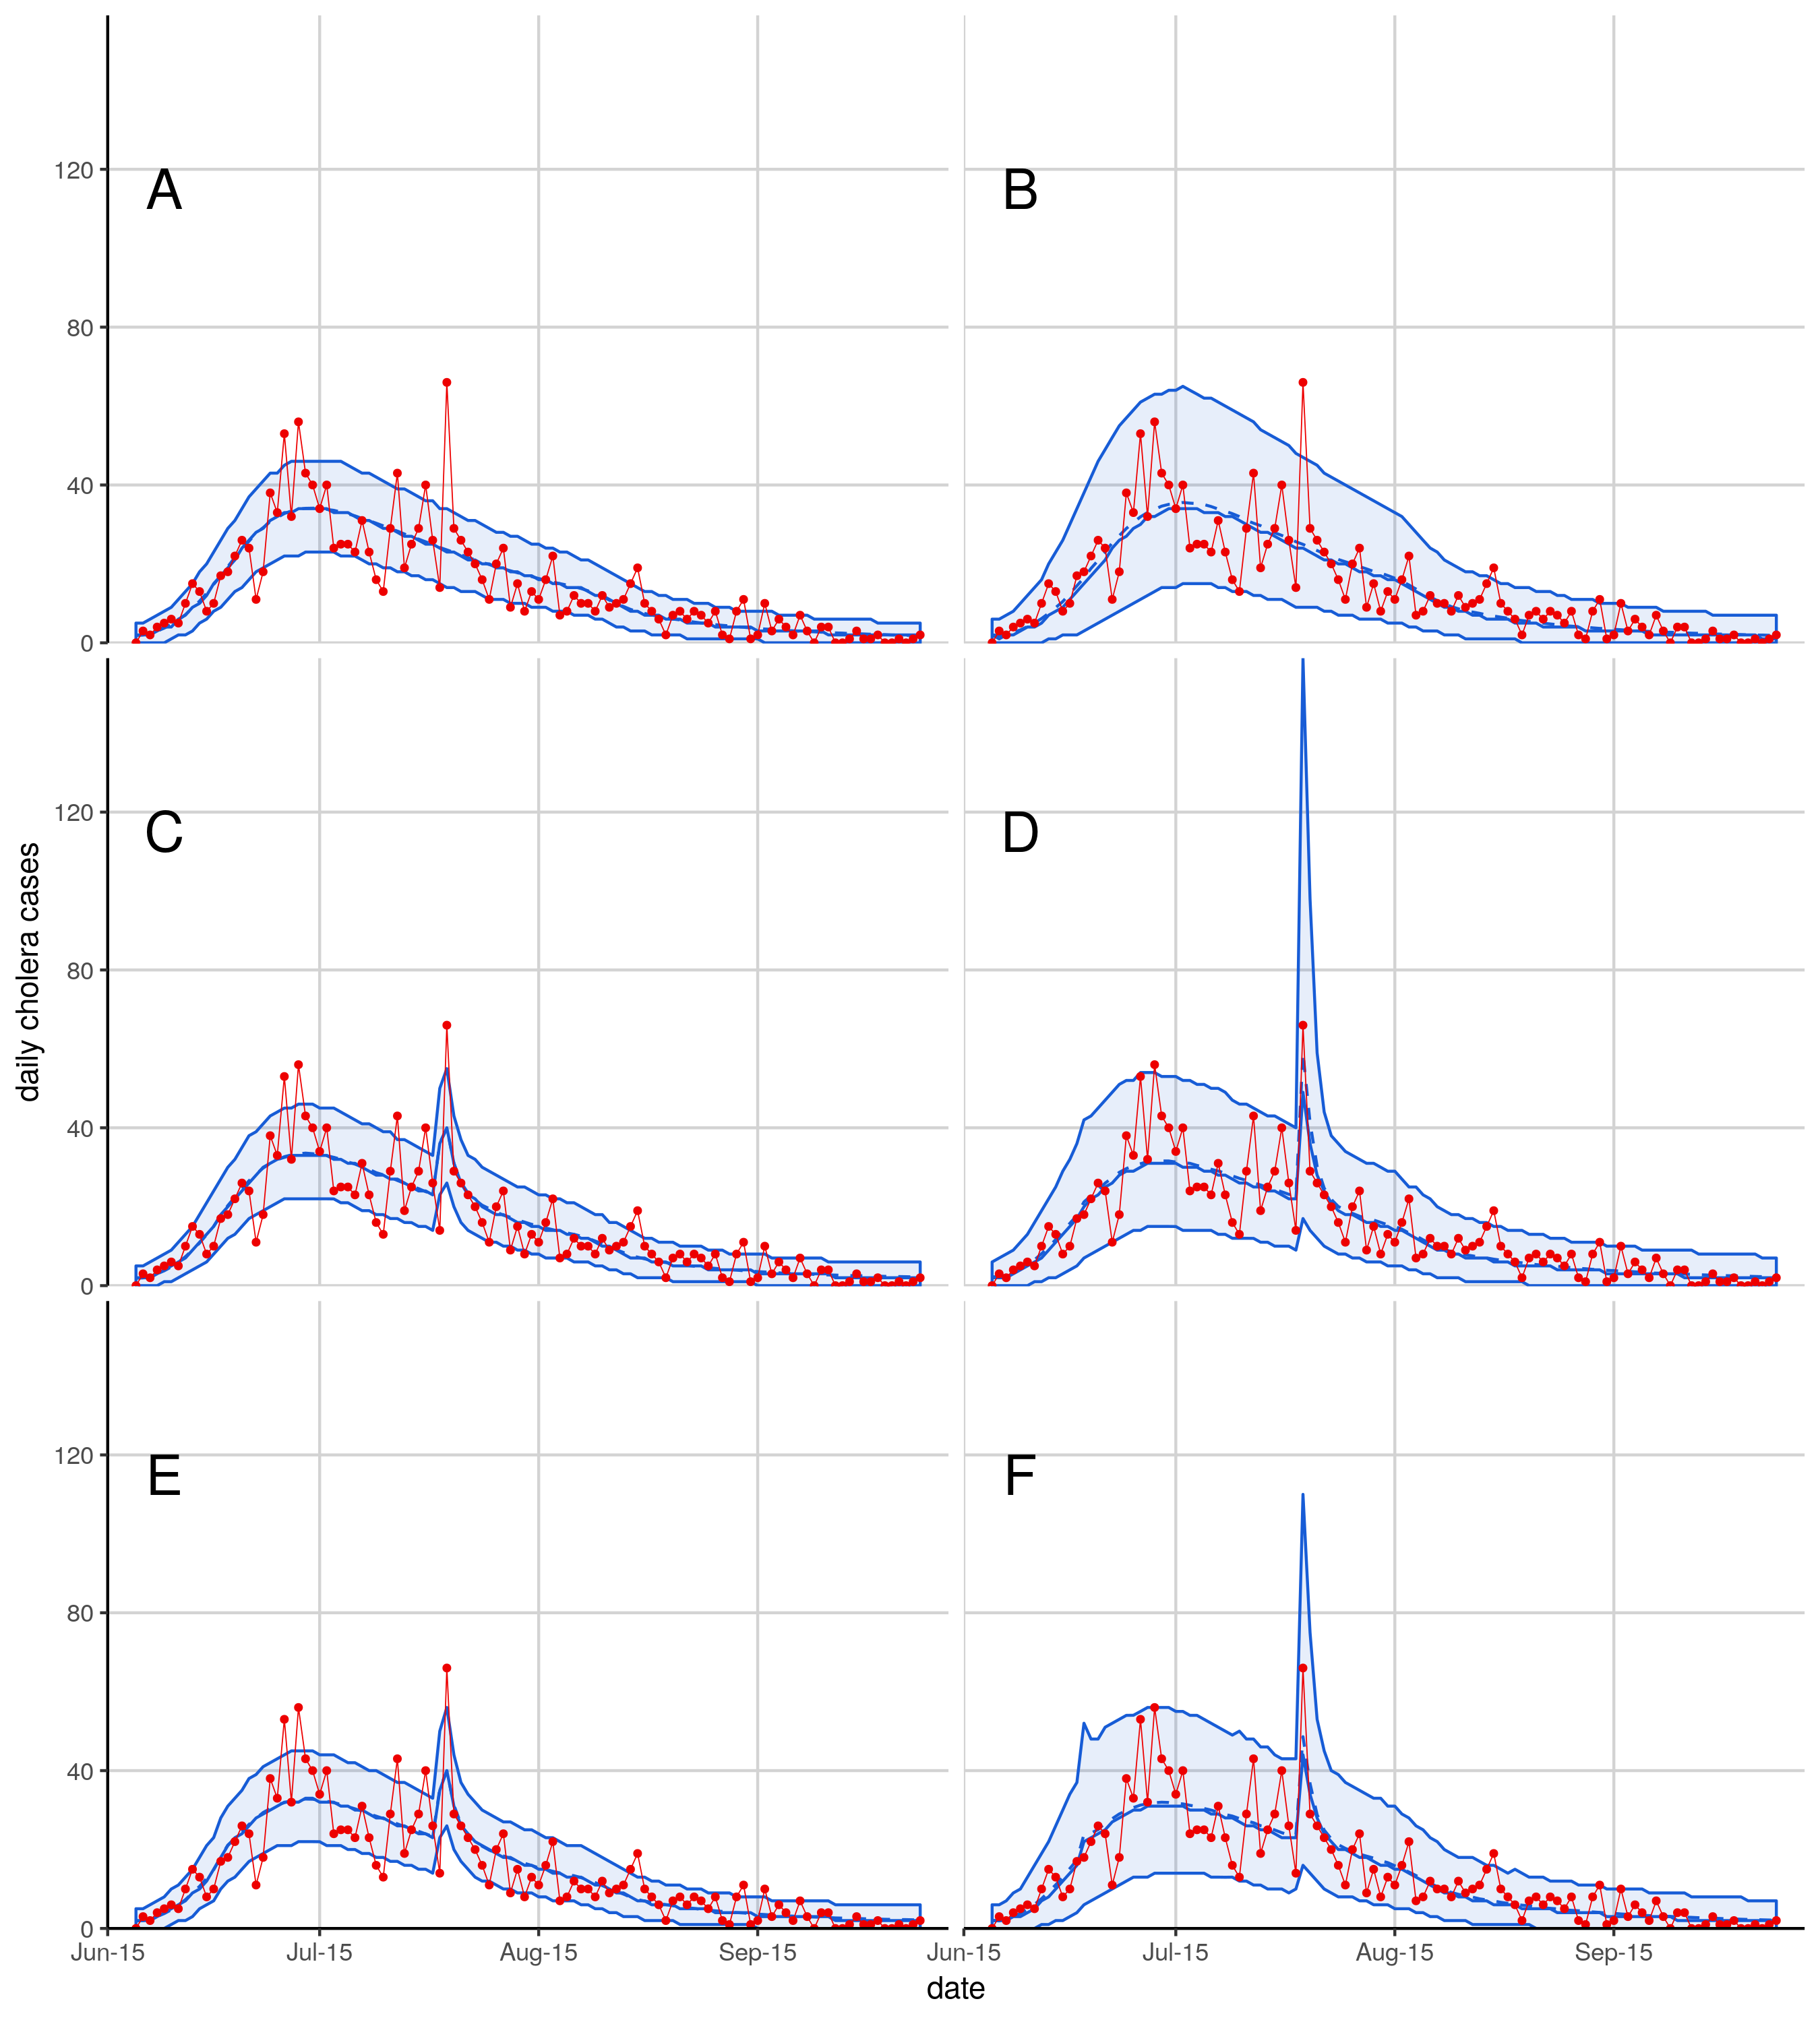
\includegraphics{fig_cholera-rainfall/Lemaitre_ACTROP_2018_42_R1_fig4.png}
    \caption[Fit of the different models]{Simulations of the \textsc{mn} (A-B), \textsc{me} (C-D) and \textsc{mec} (E-F) models. Simulations for the deterministic versions (A,C,E) are given by the mean (blue dashed line), median (blue full line) and 95\% simulation envelops (blue ribbon) of 100 simulations of the measurement model for each trajectory from 100 samples from the posteriors of model parameters against reported daily cholera cases (red line and dots). Simulations from the stochastic models (B, D, F) are given for 10'000 simulations of the stochastic process and measurement models.}
    \label{fig:sim}
\end{figure}

Comparing the two model types, stochastic results have a larger 95\% confidence interval, which better encompass most of the data. In particular, both epidemiological peaks are well captured by the stochastic models, while the deterministic results systematically underestimate them. Two factors contribute to this result: the intrinsic stochastic nature of the model, that requires the simulation of various model runs for the same set of parameters, and the noise that necessarily perturbs the force of the infection yielding an overdispersion in infections. The standard deviation of such (assumed white) noise is estimated in each stochastic model, and it is interesting to note that the MLE obtained for \textsc{ME} is slightly smaller than in \textsc{MN} (0.028 versus 0.022), highlighting again that the data are retrieved with a lower uncertainty when rainfall is included in the model. This is evident in fig.~\ref{fig:sim}, where the width of the 95\% confidence interval of models \textsc{me} and \textsc{mec} is smaller with respect to \textsc{mn}.

Finally, despite having different BFs, the deterministic models \textsc{me} and \textsc{mec} are qualitatively similar in terms of output response, indicating that the recorded changes in the log-likelihood function do not correspond to qualitative changes in the output.

\section{Discussion}
\label{sec:disc}

In this chapter, a general mechanistic SIRB-based epidemiological model is developed to evaluate the relevance of rainfall in the amplification of cholera transmission, focusing on the 2015 Juba outbreak. Two rainfall-based transmission processes were compared: the direct increase of the exposure to the contaminated water (model~\textsc{me})\cite{Eisenberg:ExaminingRainfallCholera:2013}, and the increase of water contamination by flooded open defecation sites (model~\textsc{mc})\cite{Rinaldo:Reassessment20102011:2012}. In addition, human-to-human transmission is considered (models' name with \textsc{H}).

Regarding the epidemiological model, this study introduced two innovations with respect to previous modeling attempts of cholera epidemics\cite{Bertuzzo:ProbabilityExtinctionHaiti:2016,Pasetto:RealtimeProjectionsCholera:2017}. First, the focus on daily incidence data, as opposed to weekly epidemiological reports commonly used in cholera studies, motivated the introduction of a compartment of exposed individuals, eqn.~\eqref{eq:E2j}, to account for the incubation period of the disease and, thus, the lag between the possibly rainfall-driven infection process and the manifestation of the symptoms resulting in the timeseries of daily reported cases at our disposal. %Such compartment had not been considered in previous cholera modelling works because they were most often working with weekly case reports. It was deemed necessary in this study to properly align the daily rainfall forcing with the daily reported cases.
Second, a non-linear version of rainfall driver, in the form of a power-law controlled by a single parameter, was introduced to generalize the previous linear dependence. Such formulation has the flexibility to either emphasize the impact of the largest rainfall events, or give equal weight to all non-zero rainfall intensities. %Suffice here to mention that the added parameter is properly discounted in the formal model comparison carried out here.  
%The idea is that large rainfall events may have a larger role in the deterioration of the sanitation conditions and, thus, in increasing the risk of transmission. The power low used for this goal allows, trough its parameter $\alpha$, to emphasize large precipitation events or to flatten the effect for all precipitation. 

All model assumptions were compared for both deterministic and stochastic model's types, in order to draw more general conclusions. The statistics and tests used to compare the model results  (tab.~\ref{tab:stats} and fig.~\ref{fig:lltests}) supported the significance of rainfall effects during the 2015 epidemic in Juba. In fact, results showed that for both model types there exists a significant positive effect of including rainfall drivers, in particular because standard SIRB models were not able to reproduce the second epidemiological peak of reported cases occurred in July during the recession period. All models considering rainfall, instead, showed an increase of the number of cases in correspondence of the second peak, which was due to the large rainfall rates occurred during the previous days (fig.~\ref{fig:sim}). 
This difference in the simulated responses of models considering (or not) rainfall lead to stronger support for rainfall-based models. Due to the small variations among the likelihoods of rainfall-based models, however, it is not straightforward to draw conclusions on the best way to include the rainfall effect (tab.~\ref{tab:stats}).
Models with the minimum BIC were those considering the increase in exposure (model \textsc{me}) for both the stochastic and the deterministic model types. For the deterministic models, the computation of the Bayes Factors (BFs), which should provide a direct estimation of the model probability, suggested the selection of the model combining exposure and contamination processes (model \textsc{mec}). However, this information criterion might be unstable due to numerical issues and oscillations in the \textsc{mcmc} used for calibration\cite{Raftery:EstimatingIntegratedLikelihood:2007}. By considering the fact that the models' outputs were similar for \textsc{mec} and \textsc{me} (fig. \ref{fig:sim}), it is advised to select the approach endowed with less parameters\footnote{in an attempt to maximize the model predictive accuracy we want to reduce potential overfitting.}, in this case~\textsc{me}, as indicated by the BIC. Note that the inclusion of human-to-human transmission was not statistically relevant in this modeling exercise.

\marginnote{It is also possible that the stochastic model has benefitted from improved indentifiablity. It has been shown that stochastic models can often extract more information about parameters than deterministic counterparts, see: 
\fullcite{Browning:IdentifiabilityAnalysisStochastic:2020}.}
The comparison between the likelihoods of the two models' types (deterministic and stochastic) showed that considering the stochasticity of the processes improves the model results (tab.~\ref{tab:stats}). This suggests that also deterministic models should include a stochastic term in the computation of the force of infection, eqn.~\eqref{eq:force2}, which might increase the flexibility of the outputs.

Several limitations should be considered when analyzing the present results. The calibration exercise attempted in this study considered daily rainfall and cholera reported cases, which are characterized by significant random fluctuations that might partly cloud the description of the underlying infection processes. 
Small random delays in reporting could change the infection curve and thus the effect of rainfall. This issue was partially addressed by considering the exposed compartment, eqn. \eqref{eq:E2j}, for simulation of the incubation period, and unknown reporting rate $\epsilon$ for the observed cases.

Here, it is aimed to reproduce the epidemic by modelling epidemiological transmission processes. %As usual for modelling studies, the level of description of such processes is chosen by balancing model complexity and accuracy: an increase in the number of modelled processes results in a larger number of unknown parameters, and thus a more complex calibration of the model.
While non-linear rainfall effects and possible over-reporting are taken into account, human mobility effect\cite[-4\baselineskip]{Gatto:GeneralizedReproductionNumbers:2012,Bertuzzo:SpatiallyExplicitModels:2010,Mari:PredictiveAbilityMechanistic:2015,Perez-Saez:ClimatedrivenEndemicCholera:2017} is not considered, which could help modeling the importation of infected individual.  Moreover, in this model asymptomatic infected individuals do not contribute transmission. From a modeling viewpoint, these unaccounted processes were compensated by the calibration procedure, at the loss of predictive power.

The prior bounds to be assigned to parameters are typically wide\cite{Akman:ExaminationModelsCholera:2016} because the rates governing transmission processes are highly dependent on the specific epidemiological context, so that somewhat contradictory values had been estimated in literature. These considerations, together with the intrinsic noise affecting recorded cases, underlie the possibility that some of the model parameter might be unidentifiable\cite{Eisenberg:IdentifiabilityEstimationMultiple:2013}, in the sense that different parameter combinations would yield the same model output (also called equifinality). 
The exploration of the posterior parameter distribution using an \textsc{mcmc} approach allowed us to evince the possible correlation among parameters that were well identified by the data, with the main risk of the algorithm getting trapped in a local minimum of the fitness landscape (the distribution of parameters). The posterior probability distributions of the model parameters (see the postprint supplementary information, Section S4) are associated with the model uncertainty, and were here explored by the chains of the \textsc{mcmc} calibration.

The lack of available data prevented us to include the effects of the overall efforts towards WaSH improvement in this study, but vaccination is implemented in order to eliminate one possible covariate of the rainfall effect. 
Despite these limitations, the proposed model comparison using both a deterministic and a stochastic model gave coherent results. The agreement of the two modeling types strengthened the results regarding the importance of rainfall patterns to significantly affect the development of cholera cases in time.

Overall, the findings of the study are consistent with the lessons learned in South Sudan with most of the transmission starting with the onset of the rainy season. In 2016 and 2017, cases in the dry season were observed and associated to the overexploitation of scarce water resources by nomadic herdsmen. This suggests that, as already observed, a general assessment of the relationship between precipitation and general waterborne or water-based disease infections is far from obvious and surely case-dependent. It has been argued, for example, that in the domain of water-based parasitic infections rainfall could not only boost disease transmission but also reduce it substantially\cite[-12\baselineskip]{McCreesh:ChallengesPredictingEffects:2013}, e.g. by increasing water flow (which in turn decreases habitat suitability in water). Rainfall patterns may also drastically affect human activities related to water contacts, thus potentially altering exposure and transmission risk\cite{Lai:SpatialDistributionSchistosomiasis:2015}. To that end, a hydrology-driven assessment cannot ignore certain characteristics, in particular the ephemeral or permanent nature of the waterways fostering contacts among pathogens and hosts\cite{Perez-Saez:HydrologyDensityFeedbacks:2016}. Also, temporal fluctuations of rainfall patterns may be particularly important in determining the seasonality of transmission\cite{Bertuzzo:HydroclimatologyDualpeakAnnual:2012,Bertuzzo:PredictionSpatialEvolution:2011,McCreesh:PredictingEffectsClimate:2015,Perez-Saez:HydrologyDensityFeedbacks:2016}.


%Subsuming the results obtained by this major computational exploration focused on the analysis of Juba's 2015 epidemics, it is concluded that rainfall patterns are fundamental drivers for epidemic cholera models, whether deterministic or stochastic, not only to capture seasonal trends, but also to describe short-term fluctuations in the number of reported cases. 



\part{Scientific and Public-Health response to the COVID-19 pandemic}

\chapter{Assessing the impact of non-pharmaceutical interventions on SARS-CoV-2 transmission in Switzerland}
\label{ch:covid-switzerland-npi}

%\begin{fullwidth}
\chapter[Assessing the impact of non-pharmaceutical interventions on SARS-CoV-2 transmission in Switzerland]{Assessing the impact of non-pharmaceutical\\ interventions on SARS-CoV-2 transmission\\ in Switzerland}
\chaptermark{Assessing the impact of non-pharmaceutical interventions on covid-19 transmission}
\label{ch:covid-switzerland-npi}

Following the rapid dissemination of \textsc{covid}-19 in Switzerland, large-scale non-pharmaceutical interventions (NPIs) were implemented by the cantons and the federal government between February 28 and March 20, 2020. Estimates of the impact of these interventions on SARS-CoV-2 transmission are critical for decision making in the present and future outbreaks. The aim of this chapter is to assess the impact of these NPIs on disease transmission by estimating changes in the basic reproduction number $R_0$ at national and cantonal levels in relation to the timing of these NPIs. For the whole country and eleven cantons, the time-varying $R_0$ is estimated by fitting a stochastic transmission model explicitly simulating within-hospital dynamics. The dataset includes individual-level data from more than 1000 hospitalised patients in Switzerland and public daily reports of hospitalisations and deaths. The national $R_0$ is estimated to be 2.8 (95\% confidence interval 2.1–3.8) at the beginning of the epidemic. Starting from around March 7, a strong reduction of the time-varying $R_0$ is found, with a 86\% median decrease (95\% quantile range [QR] 79–90\%) to a value of 0.40 (95\% QR 0.3–0.58) in the period of March 29 to April 5. At the cantonal level, $R_0$ decreased by between 53\% and 92\% over the course of the epidemic. Reductions in time-varying $R_0$ were synchronous with changes in mobility patterns as estimated through smartphone activity, which started before the official implementation of NPIs. Most of the reduction of transmission is inferred to be attributable to behavioural changes as opposed to natural immunity, the latter accounting for only about 4\% of the total reduction in effective transmission. As Switzerland considers relaxing some of the restrictions of social mixing, current estimates of time-varying $R_0$ well below one are promising. However, as of April 24, 2020, at least 96\% (95\% QR 95.7–96.4\%) of the Swiss population remains susceptible to SARS-CoV-2. These results warrant a cautious relaxation of social distance practices and close monitoring of changes in both the basic and effective reproduction numbers.

This chapter is based on:
\longfullcite{Lemaitre:AssessingImpactNonpharmaceutical:2020}, and J. Perez-Saez shares co-authorship of the work. It  is referred in the following as the postprint (and its supplementary information \textsc{si})
\end{fullwidth}

\section{Introduction}
As of May 13, 2020, the ongoing coronavirus disease 2019 (\textsc{covid}-19) pandemic caused by severe acute respiratory syndrome coronavirus 2 (SARS-CoV-2) has resulted in more than 4.1 million cases and 280,000 deaths globally\cite{WHO:WHOSituationReport:2020}. Independent estimates of the basic reproduction number $R_0$ for SARS-CoV-2 from the initial phases of the epidemic in China, Europe and the United States have generally ranged from 2–3\cite{Riou:PatternEarlyHumantohuman:2020} with doubling times on the order of 2–4 days. In response to the rapid increase in reported cases and hospitalisations, most countries have implemented non-pharmaceutical interventions (NPIs), including compulsory face mask use, border and school closures, quarantine of suspected and confirmed cases, up to population-wide home isolation\cite{HITCOVIDTeam:HealthInterventionsTracking:2020}. An observation study conducted in Hong Kong during this pandemic estimated that social distancing measures and school closures reduced \textsc{covid}-19 transmission, as characterised by the effective reproductive number, by 44\%\cite{Cowling:ImpactAssessmentNonpharmaceutical:2020}. Comparable reductions have been observed in many different settings\cite{Flaxman:Report13Estimating:2020}. Making decisions around relaxing NPIs requires both a careful assessment of the level of pre-relaxation transmission (e.g., $R_0$) and quantification of the expected increase in transmission from relaxation of different NPIs. 

From the initial reported case on February 24 to April 29, Switzerland reported more than 24'400 laboratory confirmed COVID-19 cases and 1'408 official deaths affecting all 26 cantons\cite{OFSP:RapportSituationEpidemiologique:2020}. The federal government issued a series of special decrees from February 28 banning gatherings of more than 1'000 people culminating on March 20 recommended home isolation (fig.~\ref{fig:covid-ch-data}). One month after the first NPI, daily confirmed case incidence had decreased from a peak of more than 1000 to a daily average of under 170 in the week of April 20–26 (fig.~\ref{fig:covid-ch-data}). Initial reports have suggested a basic reproduction number ($R_0$) of 3.5 at the start of the epidemic, with a decrease of 85\% by March 20\cite[-3\baselineskip]{Flaxman:Report13Estimating:2020}.
\begin{figure*}\centering
  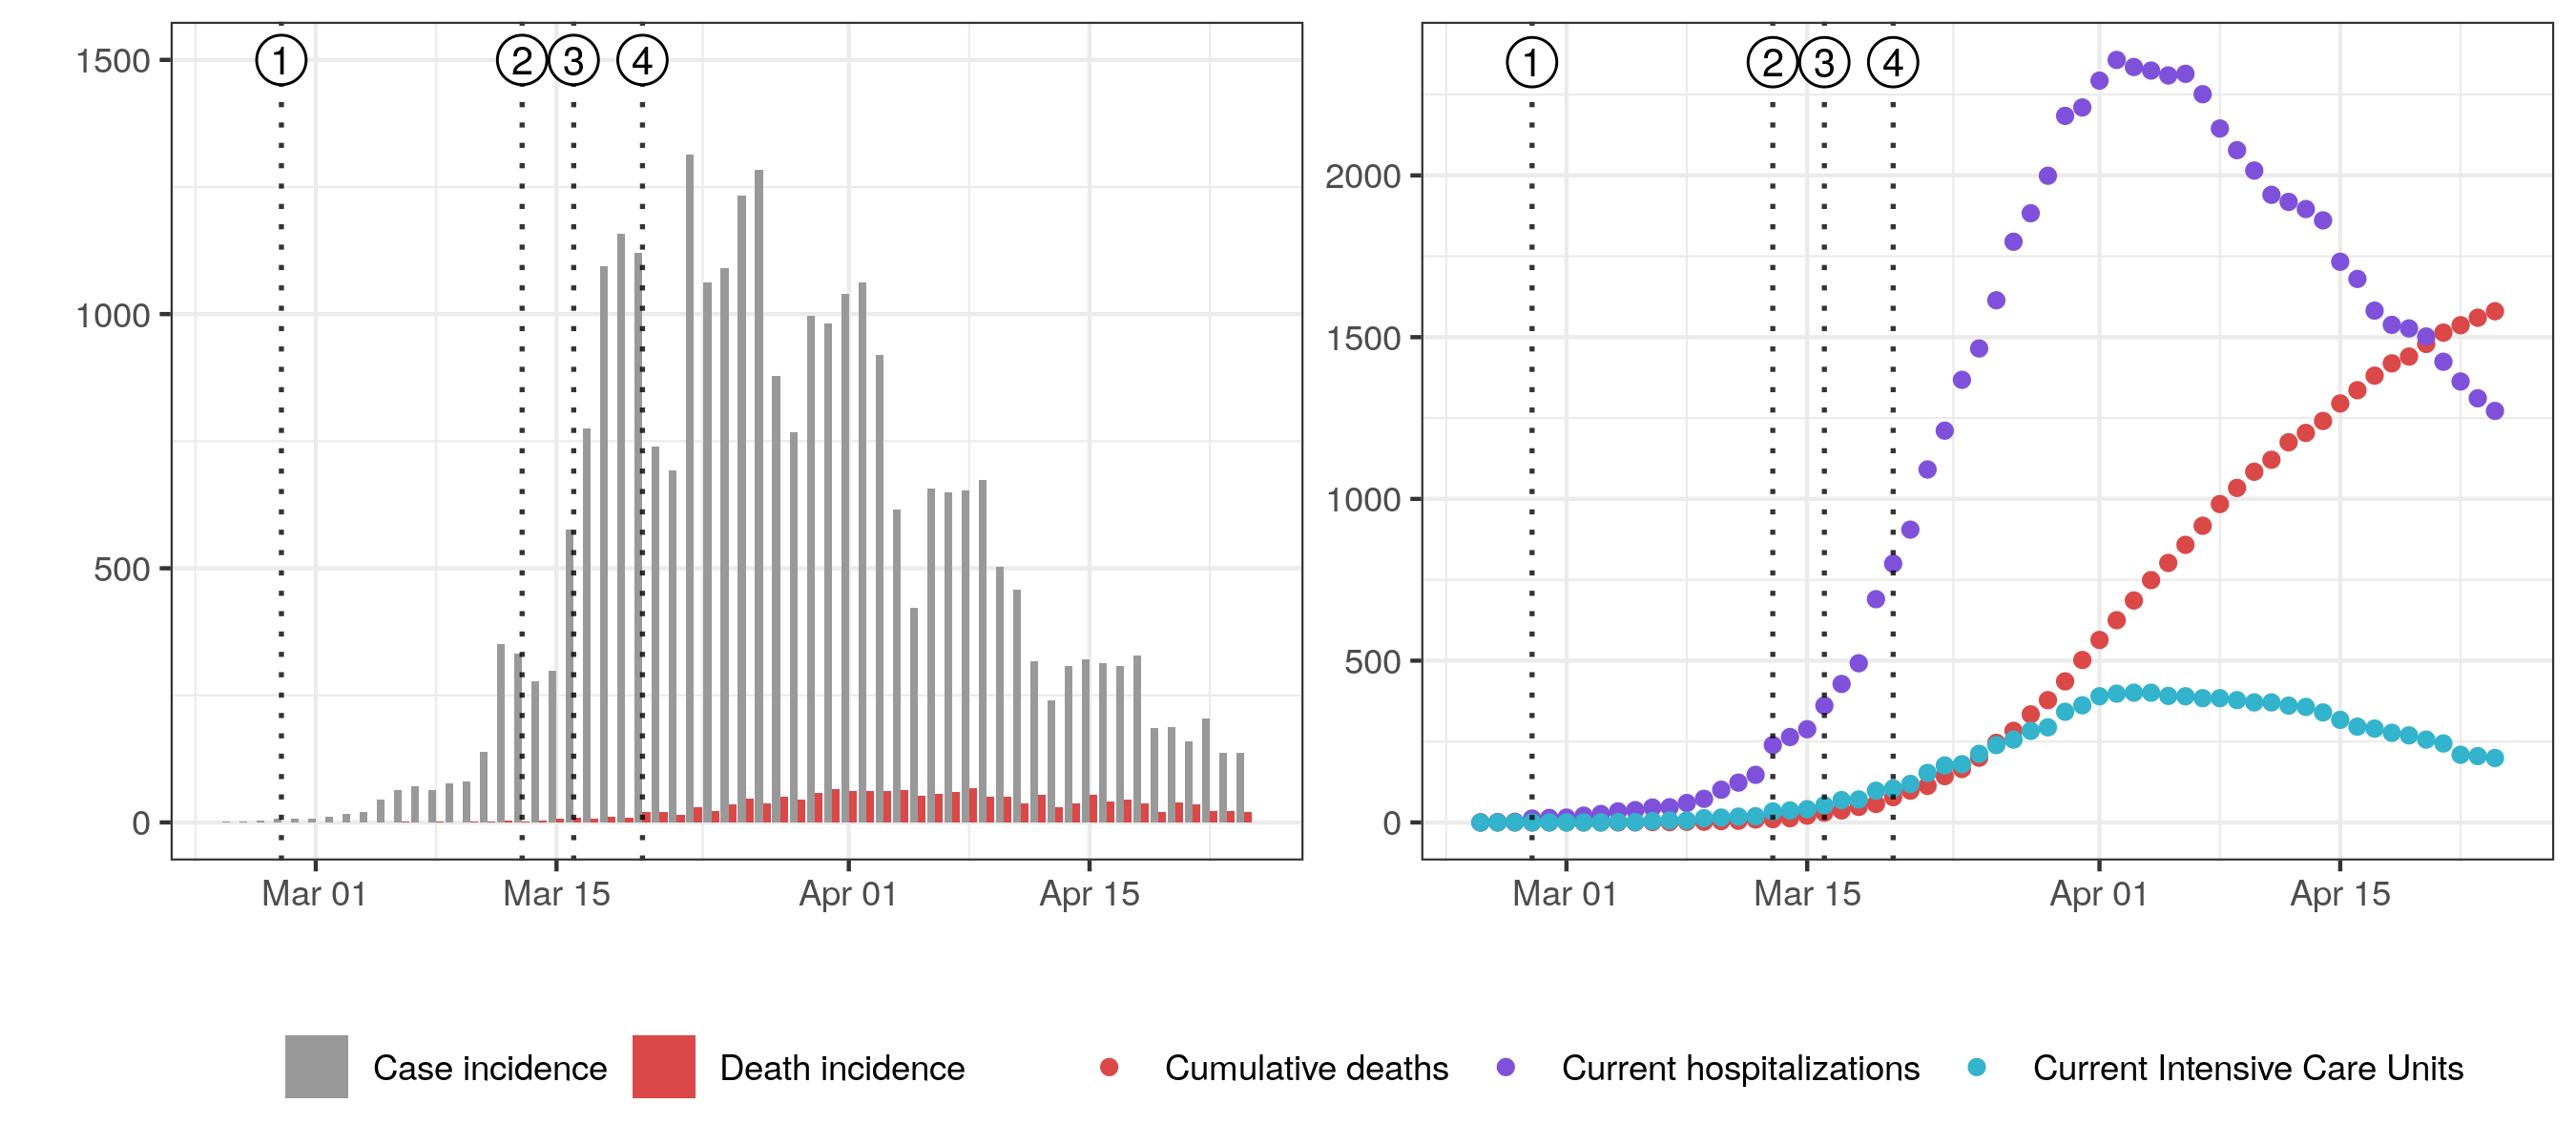
\includegraphics[width=\textwidth]{fig_covid-switzerland-npi/FIGURE_1.png}
  \caption[\textsc{covid}-19 epidemic curve in Switzerland and timing of interventions]{\textsc{covid}-19 epidemic curve in Switzerland and timing of non-pharmaceutical interventions. Dotted lines indicate the issuing of NPIs: (1) ban on gatherings of more than 1'000 people, (2) school closure, (3) closure of non-essential activities, and (4) ban on gatherings of more than five people. Left: Daily case incidence at time of reporting along with death incidence. Right: Current hospitalisations, intensive care units (ICUs) and cumulative deaths. Data from \textcite{Probst:DaenuprobstCovid19casesswitzerland:2020}, and may therefore present inconsistencies with official reports from the Federal Office of Public Health% due to reporting delays.
  }
  \label{fig:covid-ch-data}
\end{figure*}
 However, these estimates, part of a multicountry analysis of NPIs, relied on death incidence and did not account for specifics of the hospitalisation processes in Switzerland. Moreover, changes in $R_0$ were assumed to be on the date of NPI implementation, thus not allowing for the exploration of the relative timing between NPIs and changes in transmission. Furthermore, such delays likely bias the estimate $R_0$. 

NPIs affecting daily activities such as school closures and gathering bans aim at having a direct impact on mobility patterns to reduce potentially infectious social contacts. In other terms, the causal pathway from NPIs to transmission reduction is mediated by changes in mobility. Recent releases of mobility data from smartphone software providers give the possibility to study the associations between the implementation of movement-limiting measures, behavioural change and the related changes in $R_0$. Context-specific data on the degree and speed of compliance with these types of NPIs and associations with the observed decreases in $R_0$ could inform scenario-building should the future reinstatement of measures become necessary. Given that $R_0$ directly represents transmission potential, its quantification enables us to estimate the proportion of reduction in transmission attribuable to behavioral changes. In this sense, tracking of $R_0$ is more suited to study the impact of NPIs than the effective reproduction number $R_{eff}$, which is an aggregate measure of transmission capturing aspects of both infectious contacts and of population susceptibility. 

Here, the goal is to estimate the changes in $R_0$ over the course of the epidemic at both the national and cantonal levels using detailed data on hospitalisations and deaths from Switzerland between February 24 and April 24. In order to understand the estimated changes in $R_0$, its relationship with the timing of NPIs and human mobility estimates derived from cell phone data is explored.

\section{Methods}
The setting for the present chapter arose while providing scenario modeling reports, as presented in \textsc{Chapter~4}. CHUV, the hospital coordinating Canton de Vaud response, provided access to individual hospitalization data. The dataset and processing to account for right-censoring are presented in the \textsc{Appendix to Chapter~5}. This dataset allowed for refined estimates of stays in hospital and death processes, which in turn were used as assumptions in a \textsc{covid}-19 model; giving said model sufficient stiffness to estimate $R_0$ in time. Model equations and fixed and inferred parameter values are left in the postprint \textsc{si}.

\subsection{Model and assumptions}
\paragraph{Model Structure} A stochastic compartmental model of the \textsc{covid}-19 epidemic and hospitalisation processes is developed for each canton of Switzerland. The model is structured around the classical S, E, I and R compartments\cite{Kermack:ContributionMathematicalTheory:1927}, and the model diagram is shown in fig.~\ref{fig:covid-ch-diagram}. %Namely, the population is divided in compartments depending on their status with regard to \textsc{covid}-19. 
A susceptible individual $S$ might be exposed after contact with infectious $I$ individuals. Upon exposure, a formerly susceptible individual goes through an incubation period $E$ before becoming infectious $I$. The individual then recovers $R$ and does not participate in transmission anymore. 
%In addition to these dynamics, some proportion of infectected invididuals develop severe disease and among those, some are hospitalised and may advance to needing the intensive care unit. 
In addition to these dynamics, infected individuals have some probability of developing severe symptoms. Estimates derived from data from the canton of Vaud, as shown in the  show a high proportion of deaths outside of hospitals ($\approx 50\%$) hence two pathways are modeled depending if the individual seek  or has access to hospital care.  Some severly infected will be treated in a hospitals after a delay from symptom onset $I_h$. In this case, hospitalization lead to discharge (recovery) or death, either through normal hospitalization ($H_{s}$ and $H_d$ respectively) or passing through Intensive Care Units (ICUs, compartments $U_{s}$ and $U_d$ respectively). Otherwise, severly infected may recover or die without passing through hospitalization, going into compartment $I_d$. There is no need to explicitly model a latent stage where individuals are still asymptomatic but infectious\cite[-8\baselineskip]{Ganyani:EstimatingGenerationInterval:2020,He:TemporalDynamicsViral:2020, Liu:ContributionPresymptomaticInfection:2020} as only hospitalisation and death data is used. The model is implemented as a hidden markov model using the pomp R package\cite[-3\baselineskip]{King:StatisticalInferencePartially:2015}. 
 \begin{figure}[!htb]
\begin{center}
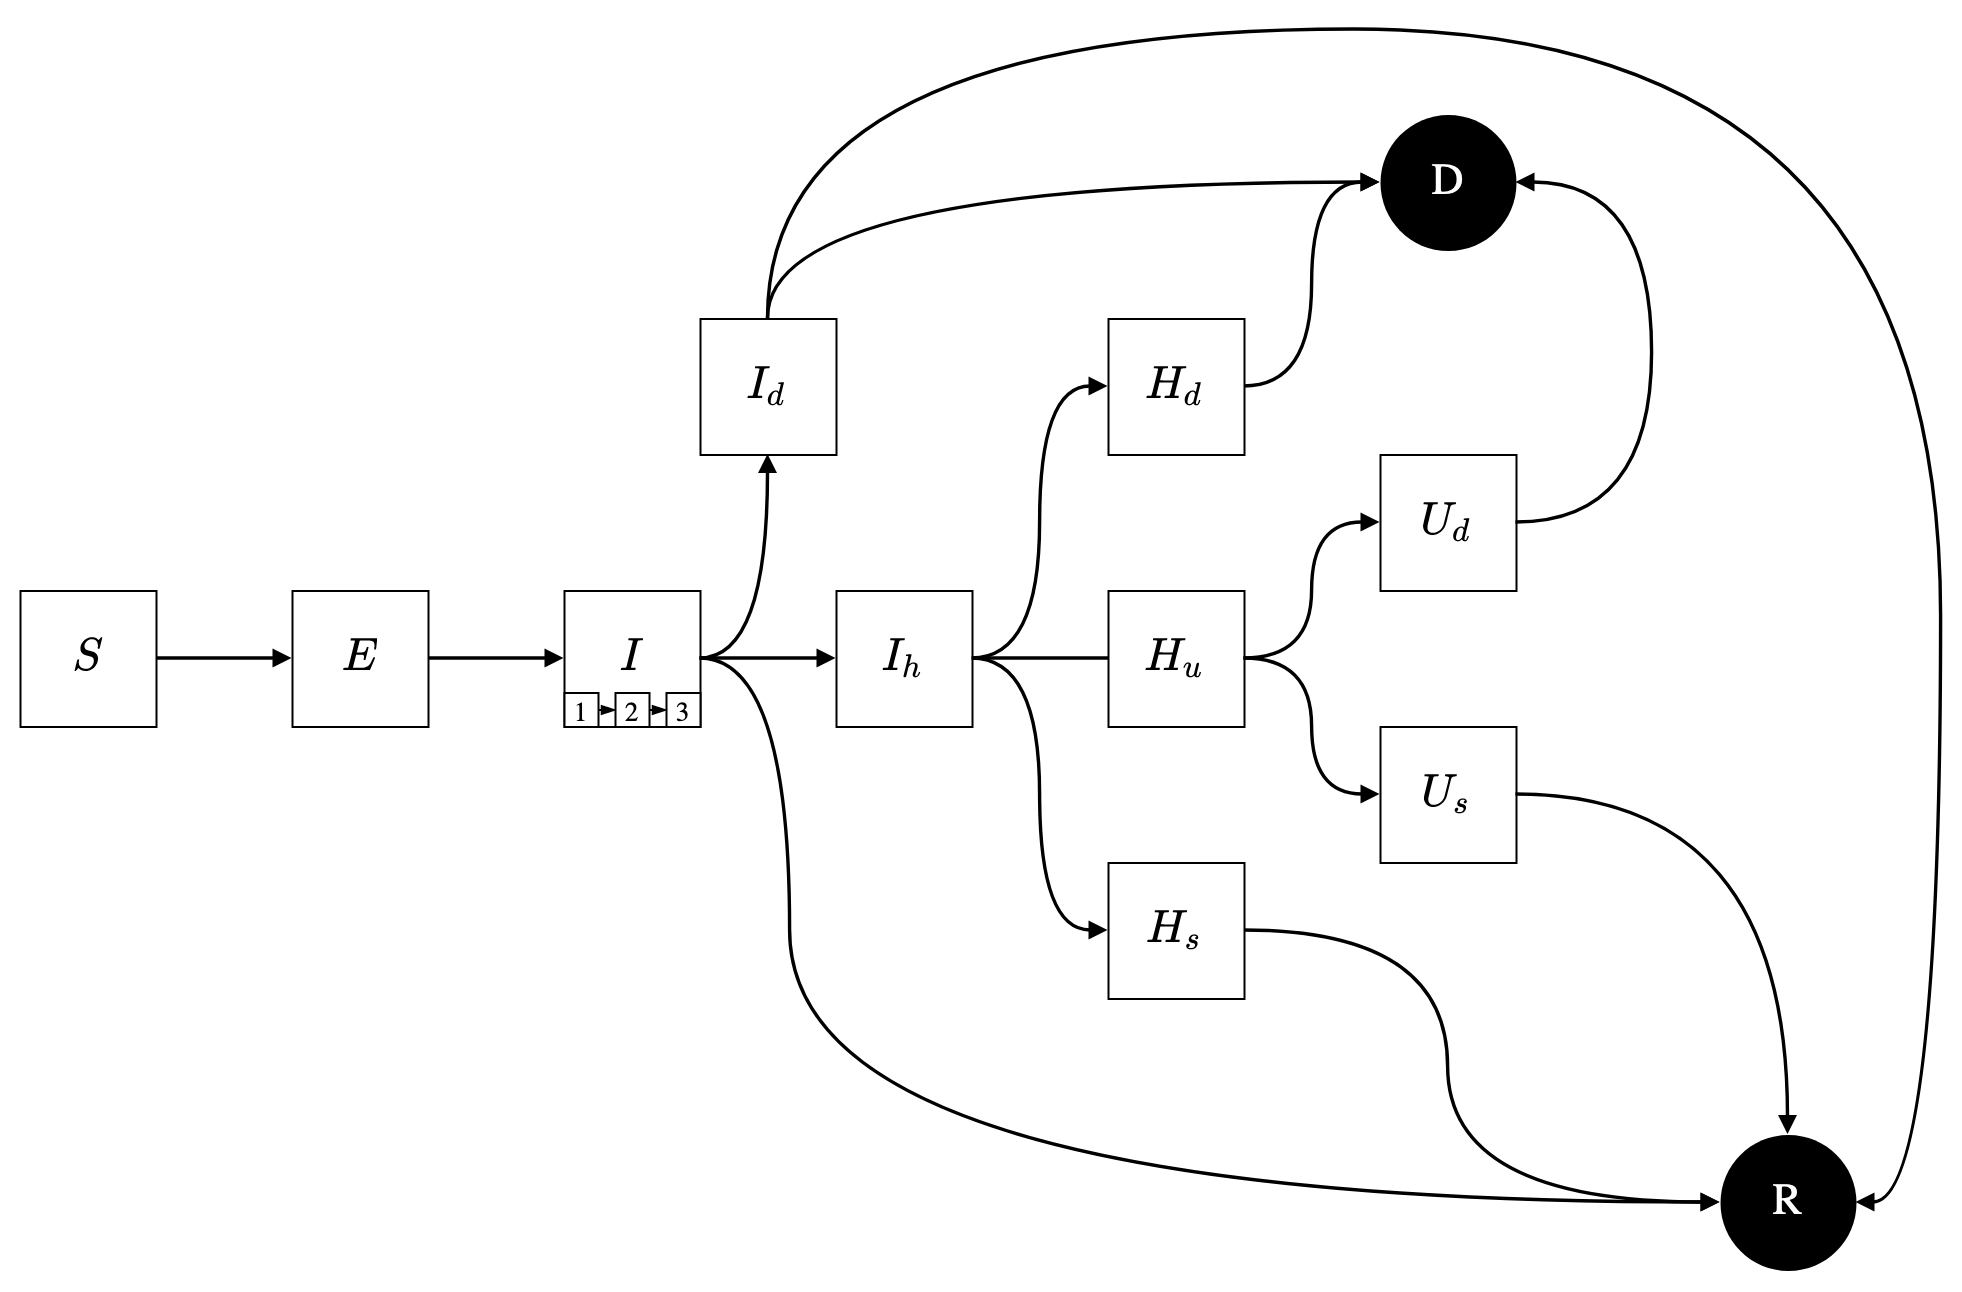
\includegraphics{fig_covid-switzerland-npi/fig_supp/diagram.png}
\caption[Schematic diagram of \textsc{covid}-19 transmission and hospitalization processes]{Schematic diagram of \textsc{covid}-19 transmission and hospitalization processes. There are two sinks: Death $D$ and recovered $R$. Each stage with regard to the disease may be implemented with several compartments (subscript numbered boxes) to better represent the time distribution spent in that stage.}
\label{fig:covid-ch-diagram}
\end{center}
\end{figure}

\paragraph{Assumptions} The reader is referred to the postprint \textsc{si} for the exhaustive description of model transitions and parameters. As parameter indentifiability is needed to capture the dynamics of $R_0$, most of the parameters were fixed to values from the litterature or obtained analyzing the data from Canton de Vaud\footnote[][-3\baselineskip]{As noted by Gostic et al., the accuracy of $R_0$ estimates obtained with the method presented here is sensible to assumptions on model structure and parameters; see \fullcite{Gostic:PracticalConsiderationsMeasuring:2020a}.}.
The transmission model is parameterized assuming a mean generation time of 5.2 days\cite{Ganyani:EstimatingGenerationInterval:2020}, and an exposed and non-infectious duration of 2.9 days\cite{He:TemporalDynamicsViral:2020}, yielding a mean duration of 4.6 days in the infectious compartments.  It is assumed that 7.5\% of infections were severe and would require hospitalisation, that 50\% of deaths happened outside of hospitals (from data on Canton de Vaud described in the \textsc{Appendix}, and data from Geneva collected from OpenZH), that 16\% of those hospitalised would die (data from Vaud, see \textsc{Appendix}), and that the infection fatality ratio (IFR) was 0.75\%, which is in the range of published estimates\cite{Verity:EstimatesSeverityCoronavirus:2020, Russell:EstimatingInfectionCase:2020}. Individual-level data on hospitalised cases from the canton of Vaud is used to estimate the distribution of time spent in the hospital and in the intensive care unit (ICU). Times to discharge and death are estimated using survival models that account for right-censoring of observations (see \textsc{Appendix}). The number of compartments for the linear-chain trick (\ie the shape parameter for the erlang distributed residence time) for each observable hospitalization state was obtained by fitting Erlang distributions to the data of canton de Vaud. To account for right-censoring the model is fitted to the estimated log-normal distributions described in the \textsc{Appendix} instead directly to observed times to events but rather. The rate parameter of the Erlang distributions is calibrated for shape parameters between $1$ and $10$ by minimizing the Kullback-Leibler (KL) divergence between the Erlang and estimated log-normal distributions. The final fit was taken to be the one with the smallest KL-divergence. We found that all hospitalization processes were best represented with exponential distributions (Erlang with shape parameter of $1$)\footnote{In the first preprinted version without the survival analysis, the shape parameters were estimated to be around 2, which highlights the importance of carefully processing data and reasoning about potential biases before using it.}.

\subsection{Data and Inference} 
\paragraph{Dataset} Curated data from OpenZH\cite[3\baselineskip]{openZH:OpenZHCovid19:2020} up to April 24 is used. This dataset included, by canton, the number of hospitalised \textsc{covid} patients, and the cumulative numbers of deaths, cases and hospital discharges; the latter not available for all cantons. The cantonal estimate is focused on cantons that had enough cases and data to obtain meaningful results, keeping 11 of the 26 cantons (Bern, Basel-Landschaft, Basel-Stadt, Fribourg, Geneva, Jura, Neuchâtel, Ticino, Vaud, Valais and Zurich). These cantons account for 66\% of the Swiss population. The national estimate uses curated national aggregate data and thus encompassed all cantons\cite{Probst:DaenuprobstCovid19casesswitzerland:2020}. Unknown parameters the model are fitted using maximum likelihood inference through iterated filtering\cite{Ionides:InferenceDynamicLatent:2015}. No attempt to include confirmed case data into the observation model were made because of the heterogeneous testing strategies adopted across cantons and over time. The model is therefore fitted to death incidence and changes in current hospitalisations using appropriate likelihood functions:
\begin{equation}
\begin{split}
 \text{deaths}(t) &\sim \text{Poisson}(\Delta D(t)) \\
\Delta  \text{hosp}(t) &\sim \text{Skellam}(\Delta H(t), \Delta D_H(t) + \Delta R_H(t)) \\
\end{split}
\end{equation}
\noindent where, $\Delta D(t)$, $\Delta H(t)$, $\Delta D_H(t)$, $\Delta R_H(t)$ are respectively the number of new deaths, hospitalized, and deaths and discharged from hospitals at time $t$, and $\Delta \text{hosp}(t)$ is the difference between the number of current hospitalizations at times $t$ and $t-1$, for which a Skellam distribution\footnote{which represents the difference between two independent random variables, each Poisson-distributed. See \fullcite{Skellam:FrequencyDistributionDifference:1946}.} is choosen. The full log-likelihood of the observation model was taken as the sum of the individual log-likelihoods of the $\Delta \text{hosp}(t)$ and of the $\text{deaths}(t)$. 
The model is calibrated separately for each canton on the daily death and hospitalization until April 24. Hospitalisation incidence data at the cantonal level would have provided more information, but this data was not accessible. Fitting to hospitalisation incidence data, which access was granted in the canton of Vaud, yielded similar results to those when changes in current hospitalisations were used. The majority of model parameters was either derived from Vaud data or from the litterature (see postprint \textsc{si}), it enables the identifiability of the reproduction number $R_0$.
 
 \paragraph{Reproduction number estimation} Time-varying basic reproduction numbers $R_0$ were estimated following a similar approach to Cazelles et al.\cite{Cazelles:AccountingNonstationarityEpidemiology:2018}, recently applied to \textsc{covid}-19 transmission in Hubei\cite{Kucharski:EarlyDynamicsTransmission:2020}. The method aims at inferring the time series of $R_0$\footnote{As mentionned, $R_0$, not $R_{eff}$ is computed as the presented method estimates the basic reproduction number, \ie the expected number of infections generate by one infected individual in a fully susceptible population. To do so, the susceptible and recovered population explicity modeled while other methods usually compute the effective reproduction number in the population by deconvolution on observed data.} that yields model dynamics that are in best agreement with the whole set of available observations. As such, the value of $R_0$ at a given point in time is informed by the whole data, and therefore does not have the limitations of being either “forward looking” or “backwards looking” as it is the case of commonly used statistical methods applied for this purpose\cite{Wallinga:DifferentEpidemicCurves:2004,Cori:NewFrameworkSoftware:2013,Lipsitch:CommentPanLiu:2020}. 
 
The model equations are similar to the previously presented partially-observed Markov Processes models, and are left in the postprint \textsc{si}. The difference lies in the force of infection. Given the state of the system at time \(t\), \(\mathcal{X}_t\), and using the same notations as in \textsc{Chapter~3}, the transition $S \longrightarrow E$ model reads:

\begin{gather}
\begin{aligned}
    \mathbb{P}\left[ \Delta N_{SE}(t) = 1 \mid\mathcal{X}_t\right] &=  \underbrace{\beta(t)  \frac{I_1(t) + I_2(t) + I_3(t)}{P}}_{\text{Force of infection} S(t)} \Delta t + o(\Delta t)\\
    \end{aligned}
\end{gather}

Time-varying $R_0(t) = \beta(t)/(3r_I)$ is modelled as a geometric random walk defined by its calibrated variance, where $\beta$ is the transmission parameter and $1/(3r_I)$ is the mean duration spent in the infectious compartments $I_1$ to $I_3$. Once the time series was inferred, the timing and slope of changes in $R_0$ is evaluated by using linear changepoint models\cite{Lindelov:McpPackageRegression:2020}. The null model corresponded to a linear decrease between two plateaus corresponding to the baseline value at the start of the epidemic and a low value after the implementation of NPIs. To allow for different slopes in the decreasing phase of $R_0$, models with one and two additional breakpoints (corresponding to two and three different slopes) are also fitted, and the best model was selected using Bayesian model selection based on leave-one-out cross-validation (details in section 6 of the postprint \textsc{si}). 

The estimated changes in $R_0$  were constrasted with changes in activity-related mobility data produced by Google\cite{GoogleLLC:GoogleCOVID19Community:2020}. Changes in activity were expressed as relative changes with respect to a baseline computed as the median over a 5-week period from January 3 to February 6. Mobility changes were computed for different categories: grocery and pharmacy, parks, transit stations, retail and recreation, residential, and workplace. Mobility estimates were based on smartphone-based geo-location location data (GPS, WiFi connections, Bluetooth) from users who activated Location History for their Google Account. These data were used to determine changes in the number of visits to and length of stays in locations categorized into the above-mentioned types. The dataset therefore only covers a sample of the Swiss population who use smartphones, the latter representing around 80\% of the total population in 2020\cite{ODea:SmartphoneUsersSwitzerland:2020}. Gaps in the dataset were filled with linear interpolation and a 7-day moving average was applied to smooth out weekly seasonality in activities. The cross-correlation between changes in $R_0$ and the averaged changes in each type of activity was computed with lags up to 10-days. Changes in $R_0$ were computed based on location-specific baselines taken as the mean value of $R_0$ from the beginning of the simulations, 5 days before the first reported case in each canton, until March 8. Changepoint models are employed identify dates of change in mobility patterns and in $R_0$. \marginnote[-5\baselineskip]{All data and code except for individual hospitalisation data from Canton of Vaud have been deposited on Zenodo (\url{doi.org/10.5281/zenodo.3862075}). The change point analysis, model fit and additional results are omitted from this thesis and may be found in the supplementary information of \parencite{Lemaitre:AssessingImpactNonpharmaceutical:2020}}


\section{Results}
\begin{figure*}\centering
  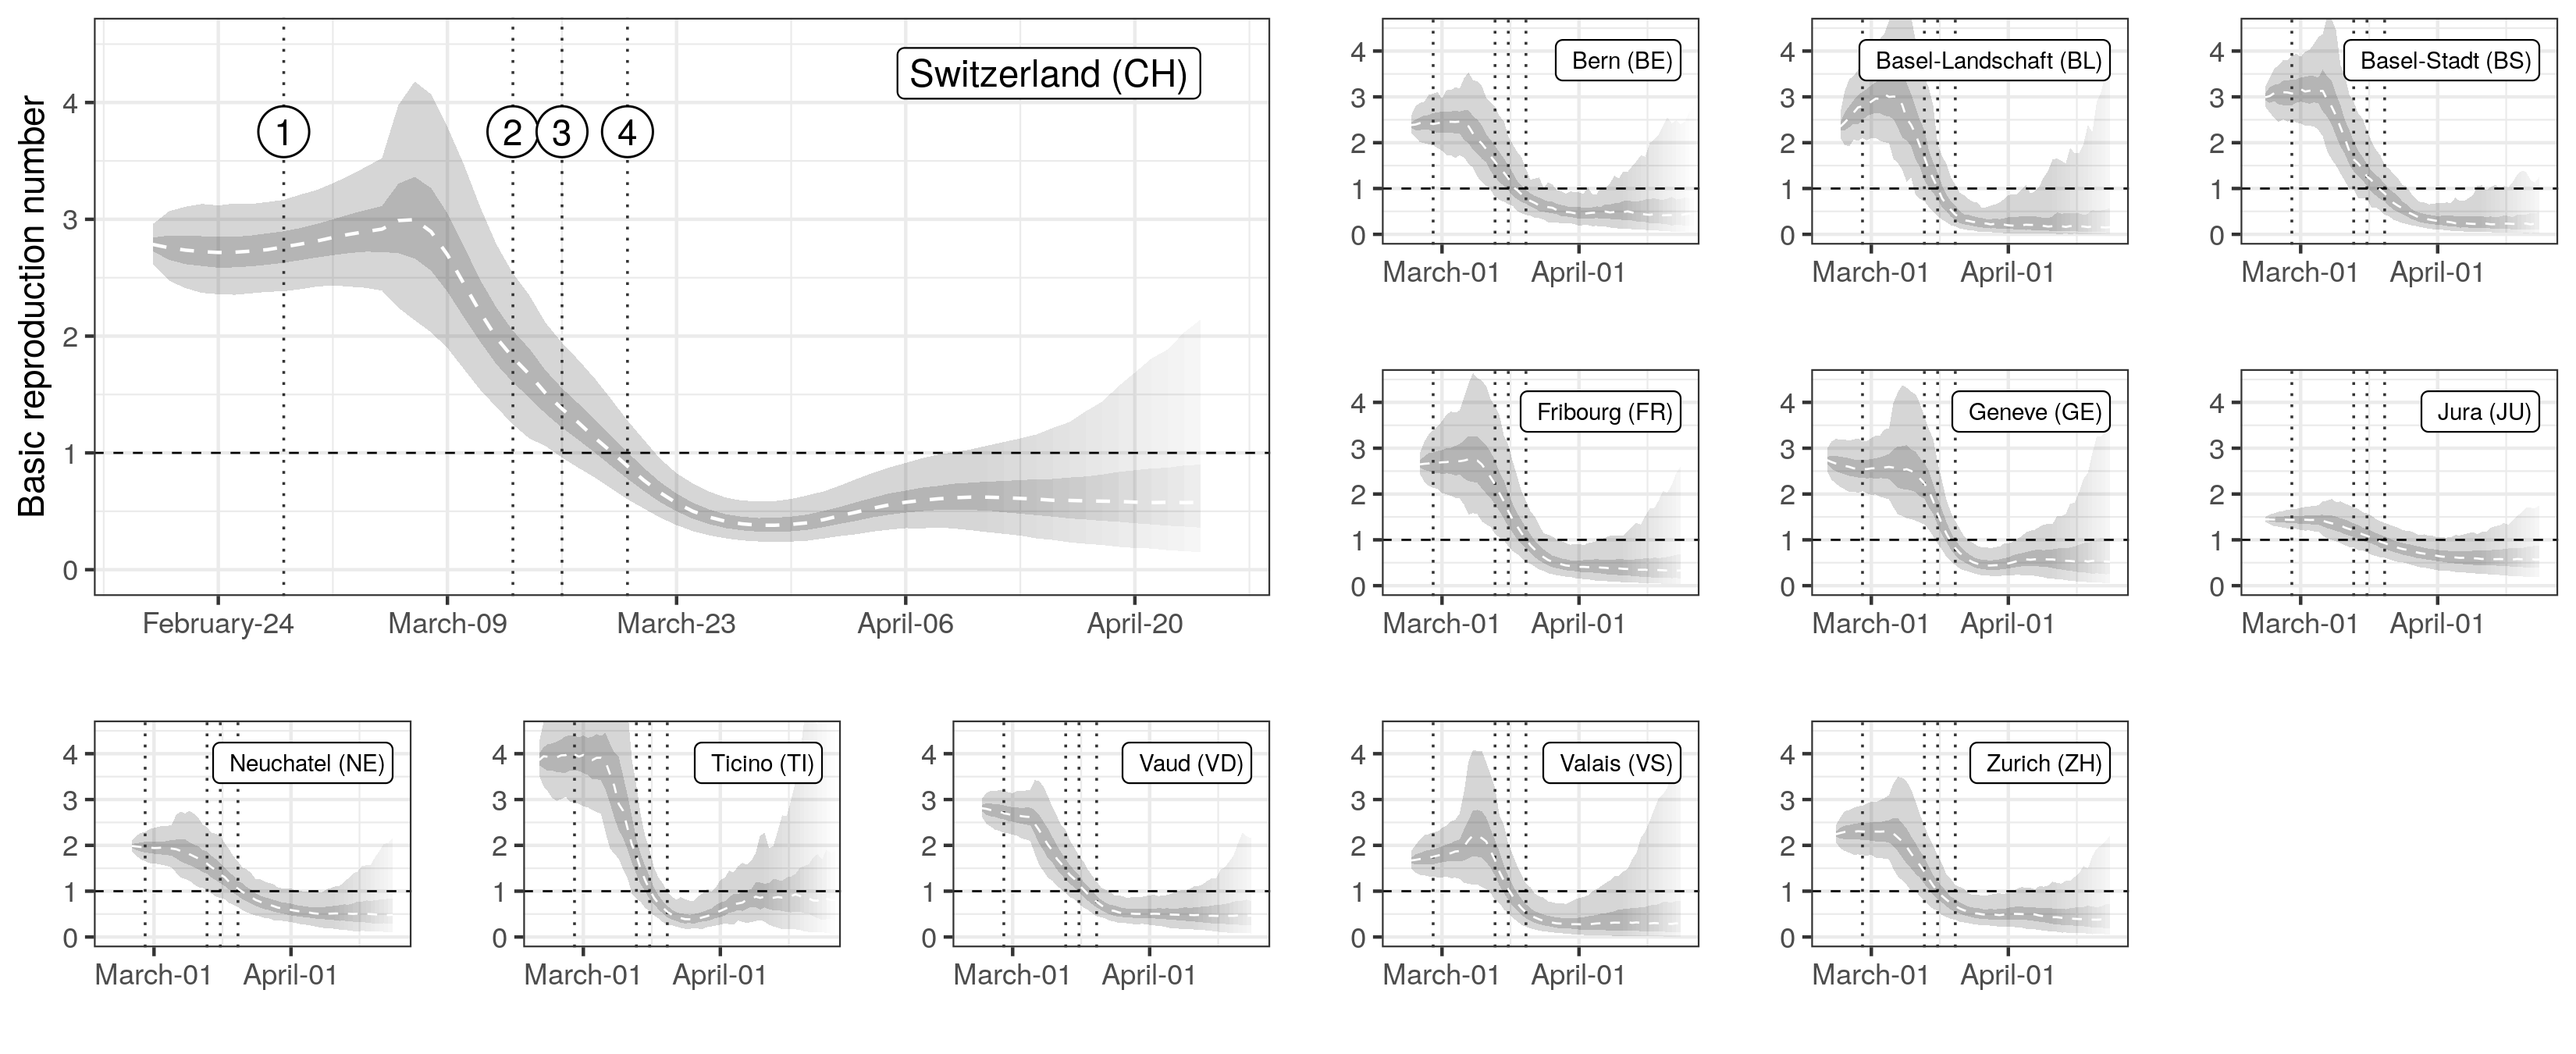
\includegraphics[width=\textwidth]{fig_covid-switzerland-npi/FIGURE_2.png}
  \caption[Estimates of changes in the basic reproduction number $R_0$][-1\baselineskip]{Estimates of changes in the basic reproduction number $R_0$. Median (dashed line), IQR (dark gray) and the 95\% QR (light gray) of the estimated time series of $R_0$ are shown for each canton. Vertical dotted lines indicate the issuing of NPIs as described in fig.~\ref{fig:covid-ch-data}. Transparency at the end of the time series indicates increasing uncertainty (style inspired by the reports of CMMID.}
  \label{fig:covid-ch-r0}
\end{figure*}
Over the study period $R_0$ trends follows a common trajectory nationally and across cantons, starting with a high plateau ($R_0 >2$) in the early stage of the epidemic followed by a rapid reduction starting at the beginning of March, and reaching a low and stable value ($R_0 <1$) from end of March onwards (fig.~\ref{fig:covid-ch-r0}). 

At the beginning of the epidemic, $R_0$ is estimated at 2.8 (95\% confidence interval [CI] 2.06–3.83) at the national level, with cantonal-level values ranging from 2.5 to 3.1 (postprint \textsc{si} tab. 5). The onset of the reduction was estimated to be between March 4 (Basel-Stadt and Vaud) and March 11 (Geneva and Valais) at the cantonal level and on March 7 at the national level (postprint \textsc{si} fig. 11). Overall a strong support is found for the reduction in $R_0$ starting before school closures on March 13 (probability 0.99 at the national level, postprint \textsc{si} fig. 11). Once started, a strong decrease in $R_0$ is estimated at the national (reduction of 0.16/day) and cantonal levels (between 0.14/day in Jura to 0.18/day in Basel-Landschaft) (fig.~\ref{fig:covid-ch-r0}). No strong support was found for changes of slope during the decrease phase at either at the national or cantonal levels except for Bern, Basel-Stadt and Vaud, for which additional changes in slopes were inferred towards the stabilisation of $R_0$ at low values (postprint \textsc{si} tab. 7).\marginnote[0\baselineskip]{Additional results may be found in the supplementary informations of \fullcite{Lemaitre:AssessingImpactNonpharmaceutical:2020}.} $R_0$ in Switzerland has been estimated to drop below 1 on March 19 (95\% CI March 16–22) with individual cantons meeting this threshold between March 16 (Basel-Stadt) and March 20 (Neuchâtel) (postprint \textsc{si} fig. 10). The probability that $R_0$ had already fallen below one was low when schools closed on March 13 (national 0.006, cantonal from $0$ in Geneva to 0.23 in Basel-Landschaft), and high by the time gatherings of five people or more were banned on March 20 (national 0.92, cantonsal from 0.52 in Neuchâtel to 0.99 in Ticino) (postprint \textsc{si} fig. 9). The estimated plateau value of $R_0$ after the reduction, that is, from March 29 to April 10, was of 0.4 (95\% quantile range [QR] 0.3–0.6) at the national level, with median values at the cantonal level ranging from 0.2–0.7 (postprint \textsc{si} tab. 5). At the national level, $R_0$ was reduced by 86\% (95\% QR 79–90\%), with median reductions ranging from 53\% (Jura) to 92\% (Basel-Stadt) at the cantonal level. A gradual reduction in $R_0$ leading to values below one around the third week of March is consistent with the observed reduction of confirmed case incidence in early April, when tarking into consideration the delays due to the incubation period, with median of 5.2 days\cite[-6\baselineskip]{Lauer:IncubationPeriodCoronavirus:2020}, and between symptom onset and reporting\cite[-2\baselineskip]{Bi:EpidemiologyTransmissionCOVID19:2020}. Similarly, the inflection in the number of current hospitalisations and ICU usage in early April also supports $R_0$ dropping below one in mid-March. 

\begin{figure*}\centering
  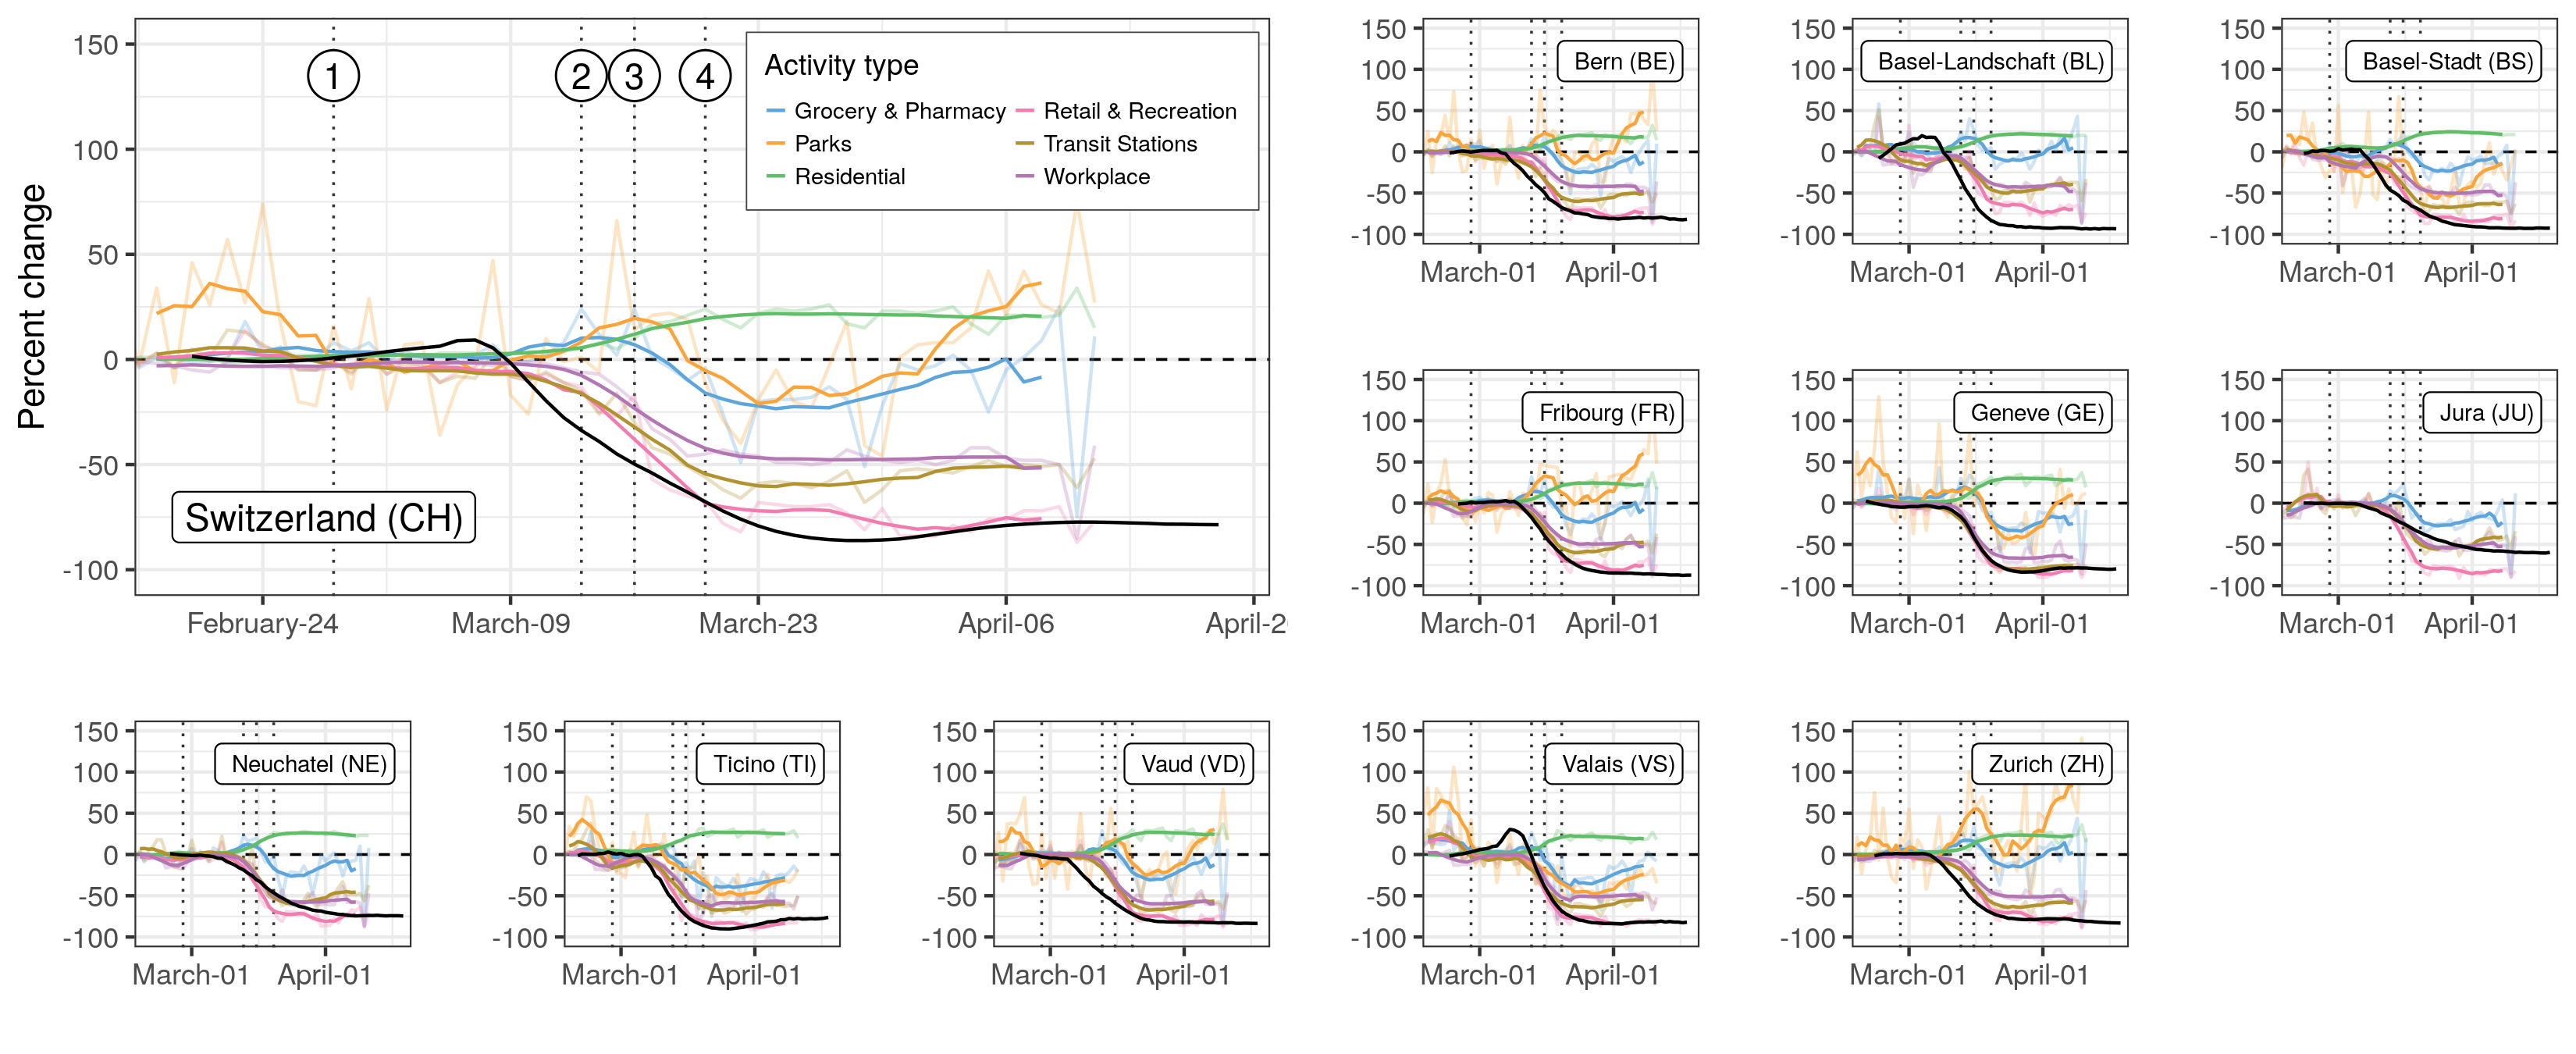
\includegraphics{fig_covid-switzerland-npi/FIGURE_3.png}
  \caption[Changes in mobility patterns and $R_0$][-1\baselineskip]{Changes in mobility patterns and $R_0$.Changes in mobility with respect to baseline are shown by activity type in terms of the daily values (transparent lines) and 7-day rolling mean (full lines), against the median estimate of $R_0$ (black line). Vertical dotted lines indicate the issuing of NPIs as described in fig.~\ref{fig:covid-ch-data}.}
  \label{fig:covid-ch-mobility}
\end{figure*}

Activity-related mobility patterns changed markedly in all cantons since the beginning of the epidemic (fig.~\ref{fig:covid-ch-mobility}). Mobility related to work, retail and recreation, and transit stations dropped by 50\% to 75\% at the national level, with cantonal-level reductions ranging from 30\% to 80\% depending on activities. Residential-related mobility increased across cantons between 20\% and 30\%. Strong support is found for mobility changes starting simultaneously for all activity types within each canton. Changes in mobility are estimated to have started between March 6 to 14 for all cantons (postprint \textsc{si} fig. 12), thus finding strong support for changes starting before school closure on March 13 (national-level mean probability across activities 0.70, cantonal range 0.55–0.99). 

Based on the changepoint models, reductions in $R_0$ likely started (probability 0.76) before observed reductions in mobility at the national level and across cantons (fig.~\ref{fig:covid-ch-mobility}). Changes in $R_0$ were highly correlated with changes in mobility, the strongest associations being with mobility related to work, transit stations, retail and recreation, and residential (cross-correlations >0.9 in all cantons and nationally, fig.~\ref{fig:covid-ch-timing}). 
\begin{figure*}\centering
  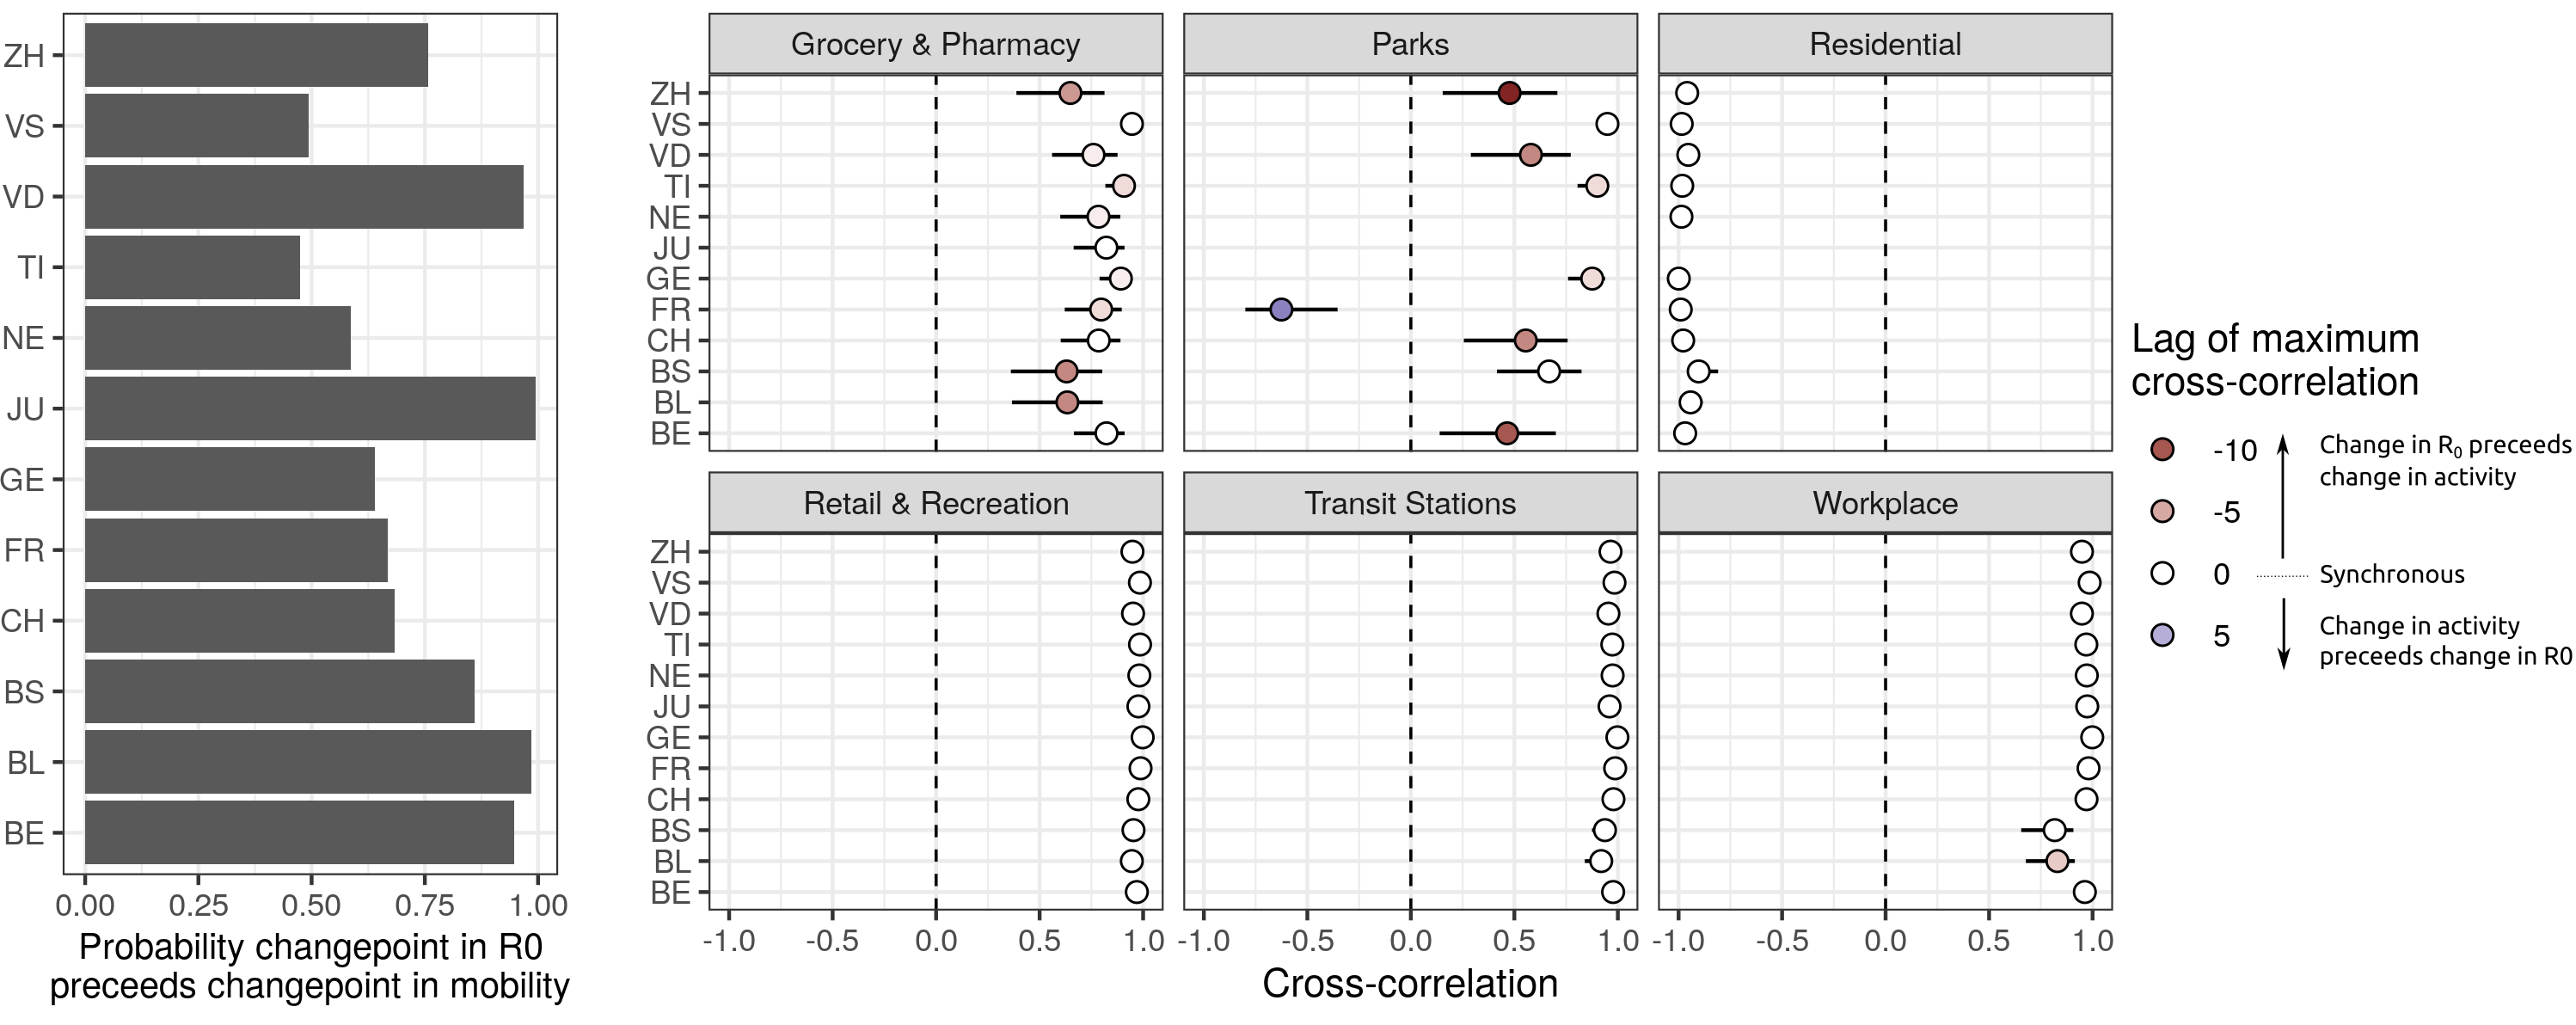
\includegraphics[width=\textwidth]{fig_covid-switzerland-npi/FIGURE_4.png}
  \caption[Timing between changes in $R_0$ and mobility][-2\baselineskip]{Timing between changes in $R_0$ and mobility. Left: probability that the first changepoint in $R_0$ occured before the first changepoint in mobility-related activity. Right: Maximum cross-correlations between time series of changes in $R_0$ and changes in mobility (bars 95\% CI). Lags refer to the delay between changes in mobility-related activity and changes in $R_0$ (positive lag k indicates that current changes in mobility have maximal cross-correlation with changes in $R_0$ $k$ days in the past).}
  \label{fig:covid-ch-timing}
\end{figure*}
In the majority of cases, correlation between mobility and $R_0$ was strongest with no lag between the two. However, changes in mobility to workplaces lagged behind changes in $R_0$ in Basel-Stadt and Basel-Landschaft. Correlations between changes in $R_0$ and grocery and pharmacy mobility were less marked (national level 0.65), with changes in mobility occurring after changes in $R_0$ (negative lags in fig.~\ref{fig:covid-ch-timing}). In most cantons, a strong increase in park mobility after March 25 resulted in a positive correlation with changes in $R_0$, but with negative lags (change in activity after change in $R_0$, fig.~\ref{fig:covid-ch-timing}). 
The linear associations between the level of reduction in mobility and maximum reduction in $R_0$ across cantons was found to be not significant, except for a small effect size for reduced park mobility (regression coefficient of 0.15, 95\% CI 0.02–0.25) (postprint \textsc{si} fig. 8). 

The effective reproduction number $R_{eff}$, a common mesure which is an aggregate measure of transmission capturing aspects of both infectious contacts and of population susceptibility was estimated. Across cantons, $R_{eff}$ was extremely close to $R_0$, indicating that a small fraction of the population is expected to have natural immunity to SARS-CoV-2. 
As of April 24, an estimated 3.9\% (95\% QR 3.6–4.3\%) of the population nationally had been infected, with median estimates ranging from 1.9\% (Bern) to 16\% (Ticino) (fig.~\ref{fig:covid-ch-map}). 
Modelled estimates of the proportion infected of people infected in the canton of Geneva are in agreement with preliminary results from ongoing serological studies, which have estimated the seroprevalence to be 9.7\% (95\% CrI 6.1–13.1\%) in the third week of April\cite[-3\baselineskip]{Stringhini:RepeatedSeroprevalenceAntiSARSCoV2:2020}, compared with modeled estimates of 8.9\% (95\% QR 7.8–10.1\%) after accounting for the time from infection to seroconversion\cite{Wolfel:VirologicalAssessmentHospitalized:2020}(postprint \textsc{si} fig. 7).

\begin{figure}\centering
  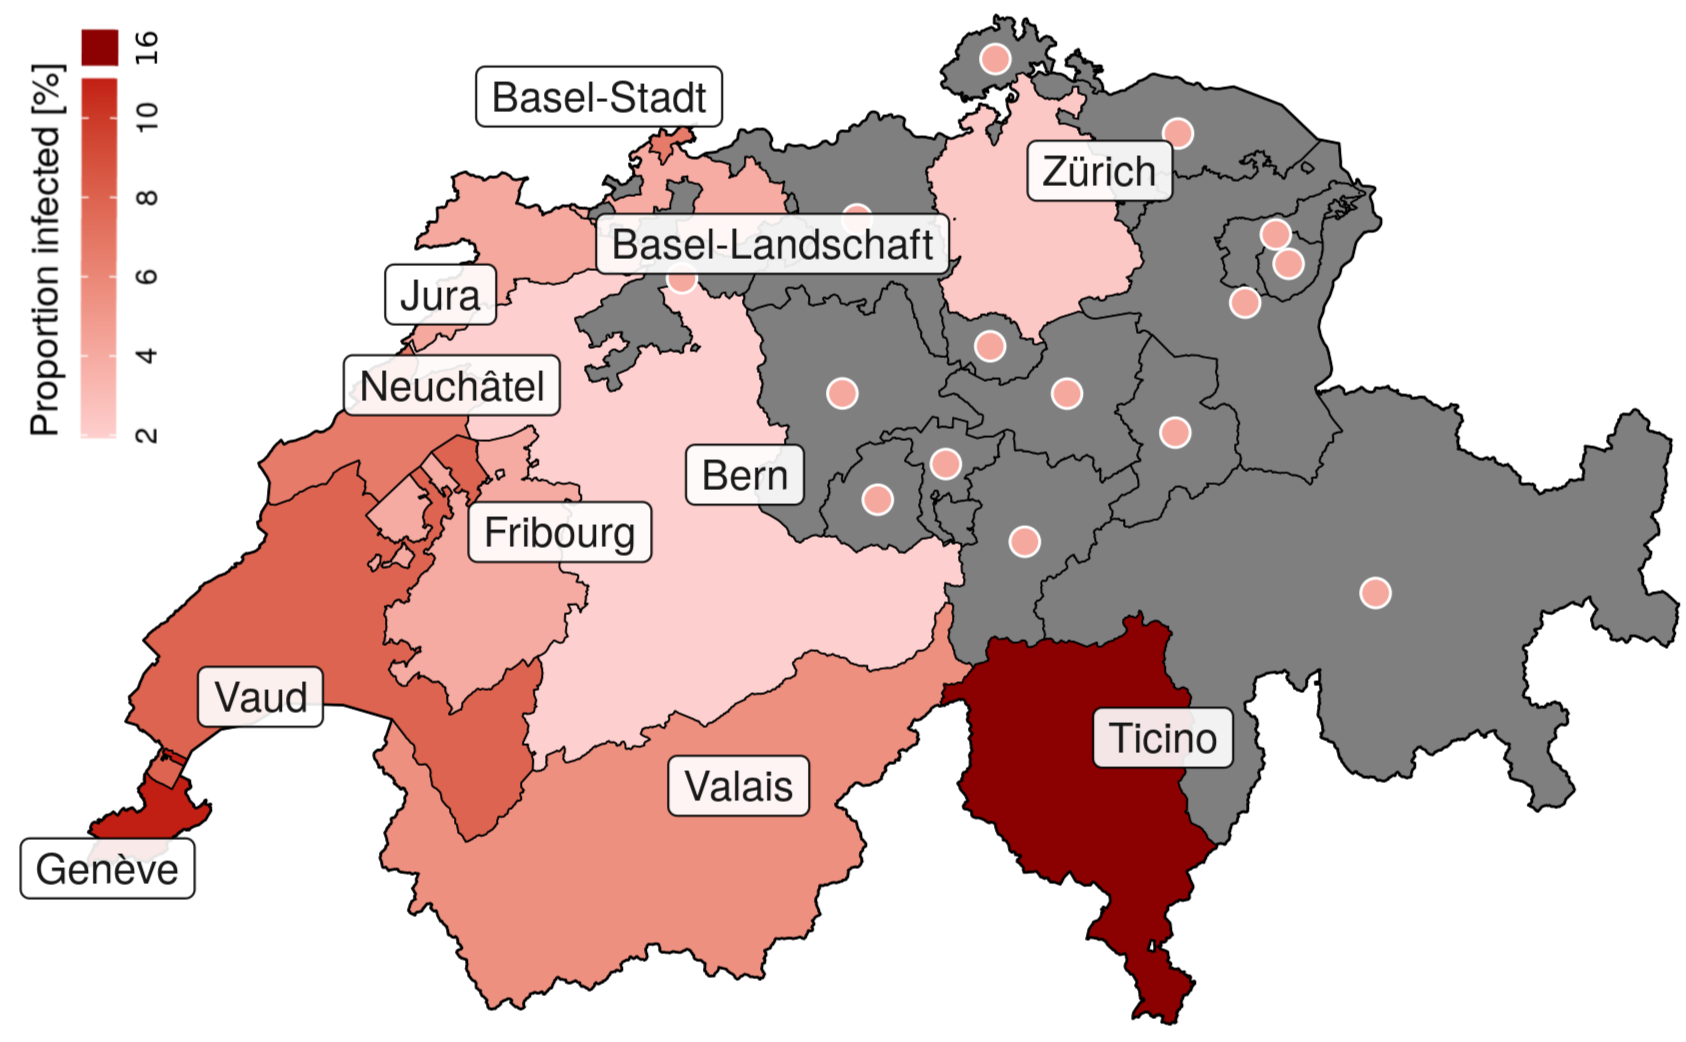
\includegraphics[width=\textwidth]{fig_covid-switzerland-npi/FIGURE_5_mod.png}
  \caption[Modelled proportion of people infected with SARS-CoV-2 in Switzerland][2\baselineskip]{Modelled proportion of people infected with SARS-CoV-2 in Switzerland up to April 24. Estimates were produced for 11 of 26 cantons for which enough data were available (unmodelled cantons are shown in gray with points indicating the national-level estimated incidence proportion of 3\%). Values are reported in the postprint \textsc{si} tab. 6.}
  \label{fig:covid-ch-map}
\end{figure}

\section{Discussion}
Our results suggest a strong reduction of $R_0$ across Switzerland since the start of the epidemic. The reduction in $R_0$ started around March 7, thus about 1 week before the implementation of lockdown-type NPIs. Analysis of activity-related mobility data also showed strong support for changes in mobility starting prior to the implementation of most NPIs. Estimated reductions of viral transmission were strongly correlated and mostly synchronous with observed changes in mobility patterns, although the initiation of changes in transmission preceded measurable changes in activity-related mobility. 

The methods used to infer the time series of $R_0$ do not rely on assumptions on the shape of how it changed in time, nor on the dates at which change started. Alternative methods that rely on fixed dates (such as that of the Imperial College \textsc{covid}-19 Response Team\cite[-6\baselineskip]{Flaxman:Report13Estimating:2020}) might be biased as changes in transmission are not synchronous with policy changes. Distribution based methods such as provided by R package EpiEstim\cite[-4\baselineskip]{Wallinga:DifferentEpidemicCurves:2004,Cori:NewFrameworkSoftware:2013} are flexible but subject to bias when misused\cite{Lipsitch:CommentPanLiu:2020}. In addition, the present approach enables the estimation of $R_0$, which is a direct quantification of transmission potential, as opposed to the effective reproduction number $R_{eff}$, which also accounts for the effect of susceptible depletion as done in the above-mentioned statistical approaches. This enabled us to estimate the proportion of reduction in transmission attribuable to behavioural changes, which is therefore more suited to study the impact of NPIs. Aside from these methodological differences, the present estimates are in line with other estimates in Switzerland: Althaus et al.\cite{Althaus:RealtimeModelingProjections:2020} estimated a reduction of 89 \% (83–94\%) from a baseline of 2.78 (2.51–3.11), Scire et al.\cite{Scire:ReproductiveNumberCOVID19:2020} estimated a reduction of 76 \% (70–82\%) from a baseline of 1.88 (1.80–1.98) and Imperial College estimated a reduction of 60\% (50–80\%) from a baseline of 3.5 (2.8–4.3)\cite{Flaxman:Report13Estimating:2020}. 

The presented results provide strong support for a reduction of transmission starting about 1 week prior to school closure, the first national-level NPI targeting daily activities, which was ordered on March 13. Moreover, initiation of transmission reduction was found to precede changes in mobility patterns as detectable from the Google dataset. A possible explanation for this initial decrease in transmission could be linked to the strong increase in public interest in \textsc{covid}-19 in February as measured by Google searches for \textsc{covid}-19-related keywords (fig.~\ref{fig:googlemob}).
\begin{marginfigure}[1\baselineskip]
%\centering
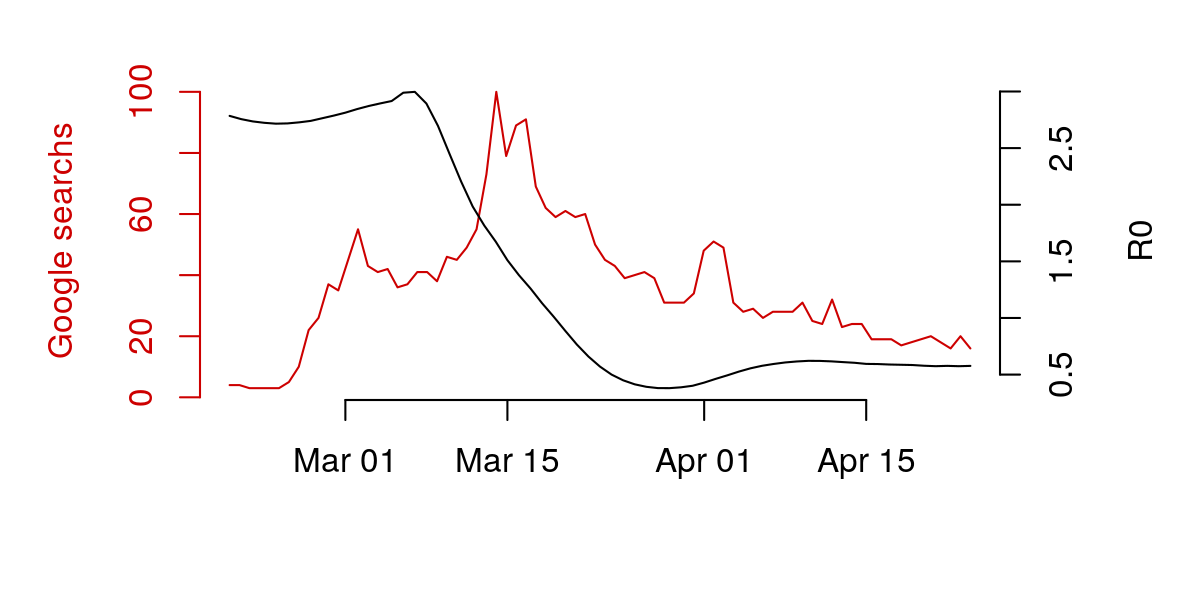
\includegraphics{fig_covid-switzerland-npi/fig_supp/google_trends.png}
\margincaption[Google trends for \textsc{covid}-19 and changes in R$_0$ in Switzerland]{\footnotesize Google trends for \textsc{covid}-19 and changes in R$_0$ in Switzerland. Trends corresponds to amount of searches for the keyword "coronavirus" (red line) between February 15 and April 30 and are given as a percent of the maximum number of searches in the period, time evolution of R$_0$.}\label{fig:googlemob}
\end{marginfigure}
 In fact, a second sharp rise in Google searches is estimated to have started on March 7 (95\% CrI March 3–9), which overlaps with the estimated start of national level decrease in $R_0$ on March 7 (probability that changepoints coincide 0.76). The Federal Office for Public Health issued an information campaign on \textsc{covid}-19 on February 28, which was updated on March 2 to stress basic hygiene rules\cite{OFSP:NouvellesReglesHygiene:2020}. This may have resulted in voluntary social distancing as well as increased hygiene early on without noticeable changes in mobility patterns. This type of proactive change in behaviour would be in line with early changes in mobility patterns, which were estimated to precede school closures and subsequent measures. The present results suggest that the value of $R_0$ was likely already below one on March 20, when the federal government banned gatherings of more than five people and recommended voluntary home isolation for the whole population. This result should however be taken within context, as the announcement was anticipated on social networks earlier that week, and so was probably already impacting social distancing behaviour. 
Therefore caution is recommend in any causal interpretation of these results on the role of this last NPI on driving $R_0$ below one.

Despite the strong association between the changes in mobility and reductions in $R_0$ within each canton, the lack of cross-cantonal associations between the level of reduction in mobility types and the level of reduction in $R_0$ suggests context-specific pathways between \textsc{covid}-19 transmission and mobility intensity. This warrants caution in attempting to apply general relations between mobility and transmission reduction. Investigation of general associations will require more in-depth studies controlling for other factors such as population density, economic activities and social mixing patterns, and inter-cantonal mobility patterns, in addition to incorporation of potential environmental drivers of transmission such as temperature and relative humidity\cite{Neher:PotentialImpactSeasonal:2020, Kissler:ProjectingTransmissionDynamics:2020}. 
  
  Several limitations to this work are noted. First, due to the relatively recent introduction of SARS-CoV-2 in Switzerland compared with the length of hospital and ICU stays, the time distribution of hospital in- and out-patients is biased towards shorter duration (see \textsc{Appendix}), which is addressed by accounting with right-censoring using survival models. In addition, because of the limited data available in some places, it was only possible to fit the model for 11 of the 26 cantons. Modelling results presented in this work are subject to hypothesis on yet uncertain parameters of \textsc{covid}-19, including the infection fatality rate and the proportion of severe infections requiring hospitalisation. An important uncertainty is the fraction of asymptomatic infections and their relative contribution to disease transmission. It is assumed that all infected individuals contribute equally to transmission, which means the estimation of the proportion of people infected would under-estimate true cumulative incidence if there were a large fraction of asymptomatic infections with a relatively low contribution to transmission. Evidence from South Korea, however, suggests that only a small fraction (2\%) of confirmed \textsc{covid}-19 infections are totally asymptomatic, and none of the household members of these asymptomatic carriers were infected\cite[-4\baselineskip]{Park:EarlyReleaseCoronavirus:2020}. Moreover, model results are in agreement with preliminary results from ongoing serological studies in Switzerland\cite[-2\baselineskip]{Stringhini:RepeatedSeroprevalenceAntiSARSCoV2:2020}.  The presented estimates of time-varying basic reproduction numbers assume that the generation interval for \textsc{covid}-19 in Switzerland remained unchanged, thus potentially ignoring the joint role of $R_0$, the infectious period and contact rates in determining the disease’s intrinsic growth rate\cite{Yan:SeparateRolesLatent:2008}. If the generation interval increased with the reduction of social contact then these estimates are conservative overestimates of the “true” value of $R_0$, which is encouraging from a public health perspective. Inferred disease dynamics and estimated time-varying $R_0$ also depend on the values of the incubation period, which is set to the estimates currently available in the literature. 
  In the present modelling framework, the initial conditions were estimated along with changes in $R_0$, which could, however, be influenced by the role of imported cases in driving disease dynamics, especially in cantons bordering regions with strong \textsc{covid}-19 transmission in early February (Eastern France for Basel-Stadt and Basel-Landschaft and Northern Italy for Ticino). 
  Since importations were not modeled, this could yield an overestimation of the initial value of $R_0$, which warrants caution in interpreting specific values of $R_0$ in these cantons. This potential overestimation would, however, not affect the strong inferred reduction in $R_0$. Another limitation of this study is that it was not possible to disentangle the individual contribution of each NPI on $R_0$ in this analysis owing to the early onset of changes in $R_0$ and in mobility patterns, as well as the very close spacing between the different types of NPI. This information would, however, be extremely valuable in supporting decisions on NPI strategies against \textsc{covid}-19. Efforts to constitute a global database of NPIs will provide the opportunity to extend this type of analysis to other settings and produce evidence for the effect of different types of NPIs\cite{HITCOVIDTeam:HealthInterventionsTracking:2020}. 
  
  As the Swiss government plans to gradually lift restrictions, close monitoring of changes in $R_0$ is critical, given that the reductions in transmission appear to be almost entirely driven by changes in behaviour, not through herd immunity. Near real-time estimates of $R_0$ may serve as a critical tool for public health and political decision makers in the months to come, and efforts should be made to refine models like ours using new data, including those from population-based serological studies, mobility data and more detailed individual-level data on \textsc{covid}-19 cases across the spectrum of severity.\marginnote[-4\baselineskip]{While relying on hospitalization and death allowed for an early robust identification of the basic reproduction number, it would be necessary to add a reporting process and case data to update this estimate through 2020-2021. Methods based on observed data are easier to maintain, and reliable continuous updates of the reproduction number in Switzerland available on the Swiss National \textsc{covid}-19 Task Force website \url{sciencetaskforce.ch/en/current-situation/}. It is provided by the ETHZ, with method described in \fullcite{Huisman:EstimationWorldwideMonitoring:2021}. The modeled incidence from the present Chapter has been later used as "truth" to compare waste-water data with reported cases, see: \fullcite{Fernandez-Cassi:WastewaterMonitoringOutperforms:2021}.}




%%
% The back matter contains appendices, bibliographies, indices, glossaries, etc.

\backmatter

% \bibliography{sample-handout}
% \bibliographystyle{plainnat}


\printindex

\end{document}

